% ===================================================
% CHAPITRE 16 — CURÉS D'OUROUX
% Pages imprimées 96-140 — vues 99-143
% ===================================================
\chapter{Curés d'Ouroux}

% --- Page imprimée 96 — vue 99
\begin{figure}[ht]\centering
    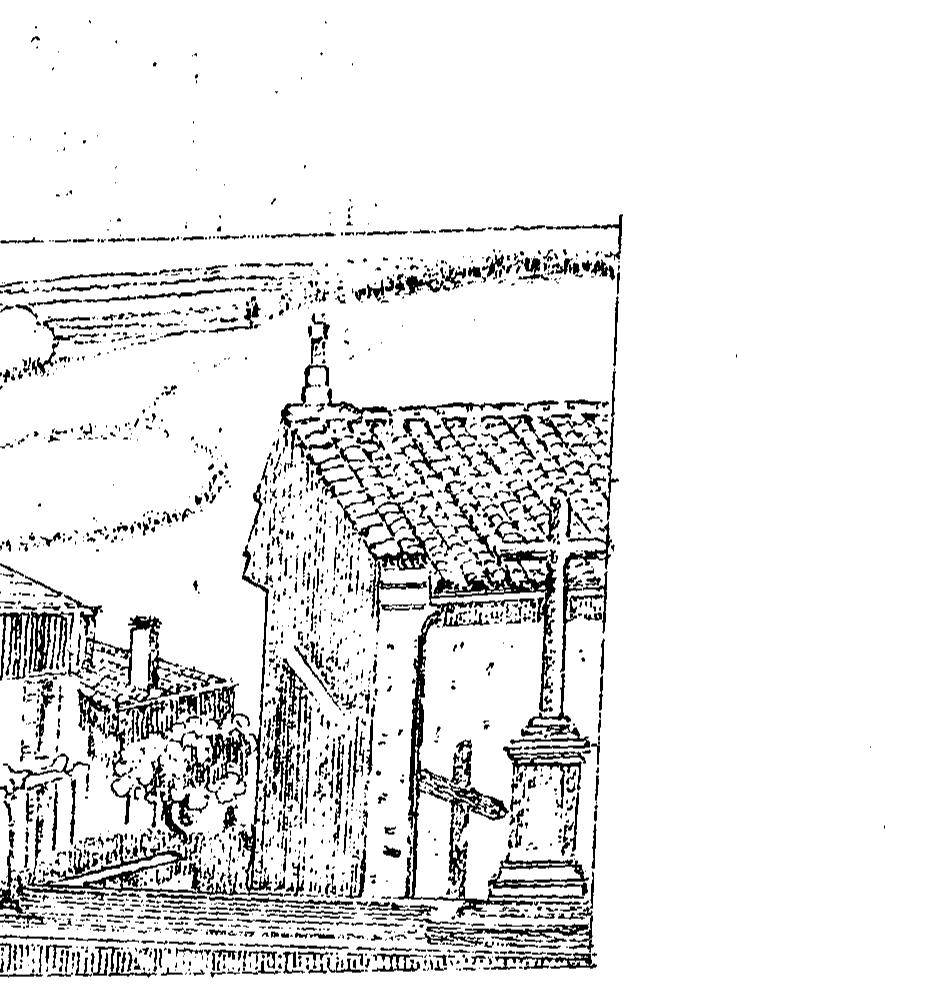
\includegraphics[width=0.55\textwidth]{Illustrations/illus-cures-vue96.png}
\end{figure}

La Paroisse St-Antoine d'Ouroux fit partie du diocèse de Macon jusqu'au 29 Novembre 1801. Le Souverain Pontife Pie VII ayant, à cette époque, établi une nouvelle circonscription des diocèses de France, le Beaujolais fut compris dans le diocèse de Lyon.

La Cure avant la Grande Révolution était de la collation du Chapitre de St-Pierre de Macon. Le titre portant nomination de Mr Trouilloux à la cure de la paroisse nous indique la procédure suivie à cette époque.

% --- Page imprimée 97 — vue 100
"Pardevant nous notaire royal et apostolique au baillage et diocèse de Macon... est comparu haut et puissant seigneur Messire Pierre Louis François de la Tour de Gouvernet, prêtre comte et prévôt du Chapitre noble de l'Esglise St-Pierre dudict Macon et l'un de messieurs les vicaires généraux de ce diocèse.. étant en sa dicte qualité de prévôt nominateur du bénéfice cure de la paroisse St Antoine d'Ouroux en Beaujolais, lequel informé de la vacance dudict bénéfice cure par le décès de Mr Antoine Guillin Dumontet Archiprêtre de Veaurenard, curé de la paroisse de St-Antoine d'Ouroux... étant bien informé des bonnes vie et mœurs, suffisance et capacité de Mr François Trouilloux vicaire actuellement demeurant la dite cure où il demeure de plein gré a nommé et présenté à Mgr l'Illustrissime et révérendissime Évêque de Macon ; le dict François Troulloux pour être par luy pourvu, tenir et posséder le dit bénéfice cure... affirmant le dict Seigneur prévôt qu'en la présente nomination, il n'est intervenu, y n'interviendra aucuns dols, fraudes, simonies ny autres pactions illicites contraires aux saints Canons.... etc."

\clearpage
\begin{wrapfigure}{l}{0.40\textwidth}
    \vspace{-0.5\baselineskip}
    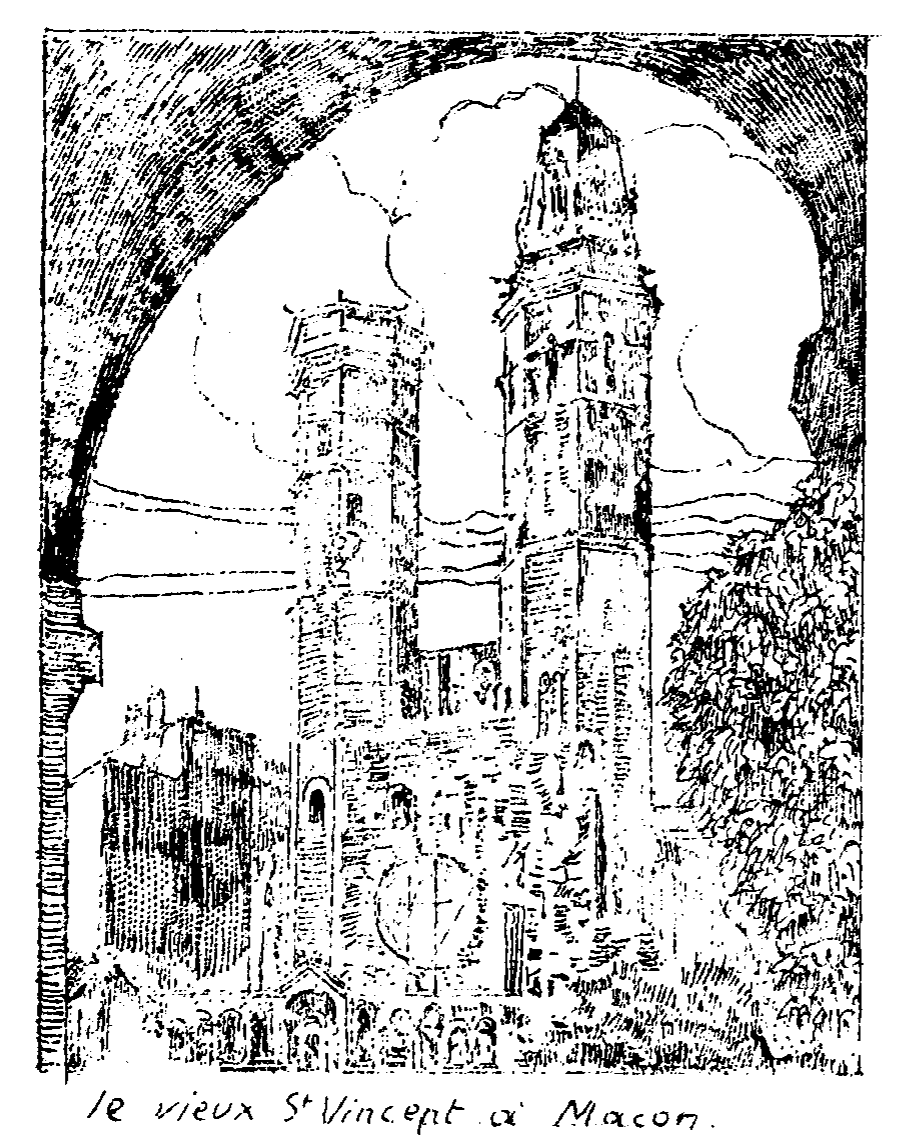
\includegraphics[width=0.37\textwidth]{Illustrations/illus-cures-saint-vincent.png}
\end{wrapfigure}

Cette union de la paroisse d'Ouroux avec la collégiale de St-Pierre remontait à une haute antiquité, puisque dès l'an 1096 le pape Urbain II, qui avait été moine de Cluny, confirma au prieur et au monastère le droit de nommer à cette église paroissiale. Aussi lisons-nous dans le

Pouillé de 1513 : "Archiprêtré de Vauxrenard. Cet archiprêtré comprend dans ses limites les églises suivantes :... Ouroux qui a été uni depuis longtemps à la mense du prieur de St-Pierre de Macon.

Comme on le voit, dans le principe, le prévôt de St-Pierre
% --- Page imprimée 98 — vue 101 (suite)
était curé né d'Ouroux. Il avait quatre prêtres sociétaires, portant le titre de vicaires perpétuels pour desservir cette paroisse ainsi que St-Jacques-des-Arrêts, son annexe. Le prévôt de St-Pierre se démit de ce bénéfice par suite de transaction au commencement du XVIIe siècle et le Chapitre conserva la collation c'est-à-dire le droit de présenter à l'évêque de Mâcon le prêtre qui devait être nommé curé.

Depuis longtemps les dîmes d'Ouroux appartenaient au chapitre de Beaujeu, in solidum. Guichard III, seigneur de Beaujeu eut pour fils Louis qui fut chanoine et chantre au chapitre de Lyon, puis évêque de Bayeux. Ce dernier ayant légué au chapitre de Beaujeu 100 sols de rente, Humbert son frère l'échangea contre la dîme d'Ouroux. Les vicaires perpétuels recevaient le tiers de cette somme et le chapitre les deux autres tiers. Le 7 Août 1664 le chapitre de St-Pierre céda ce tiers à Mr Morin, curé d'Ouroux qui le transmit lui-même au chapitre de Beaujeu par acte du 22 Novembre 1667. Depuis cette époque le curé fut réduit à la portion congrue. Cette portion congrue était de 300 livres avant l'édit du 13 Mai 1768 qui la porta à 500 livres.

Bien que le nombre de prêtres sociétaires fût de quatre, il ne paraît pas qu'ils aient jamais résidé ensemble dans la paroisse. L'un d'eux, néanmoins, pouvait résider habituellement à St-Jacques. Mr Morin (1664-1676) est le premier qui, par suite des transactions passées avec le chapitre de St-Pierre ait pris le titre de curé. Ses prédécesseurs employaient exclusivement celui de vicaire perpétuel.

Il y avait autrefois des moines de St-Bernard à Ouroux, d'après le témoignage de l'auteur du manuscrit de la bibliothèque de Lyon. Mr de Lacarelle ajoute : "nous avons sur ce couvent peu de détails. Le fait de son existence est seulement constaté par quelques actes qui subsistent encore et par les vestiges de leur maison. Des fouilles opérées près de la cure ont fait découvrir les fondations d'un bâtiment de 40 mètres environ de longueur sur une largeur proportionnée."

Cette communauté existait au XIIIème siècle. À quelle époque cessa-t-elle d'exister ? Quels furent les motifs de sa suppression ? Je l'ignore ; je n'ai du reste trouvé aucune trace de ces titres dont parle Mr de Lacarelle. Quant aux fondations, elles sont disparues en
% --- Page imprimée 99 — vue 102 (suite)
tièrement à cette heure.

Comment expliquer la présence des moines de St-Bernard dans notre vallée, aux portes même de l'illustre abbaye de Cluny? L'histoire de nos contrées pourrait nous fournir peut-être une réponse à cette question.

L'évêque et le chapitre de Mâcon entretenaient des relations peu sympathiques avec cette abbaye dont les privilèges allaient chaque jour s'accroissant davantage. Nous savons d'ailleurs que les disciples de St-Bernard protestaient par leurs austérités et leur amour de la pauvreté contre le luxe des Bénédictins de Cluny. Ouroux dépendant directement de Mâcon, offrait une position exceptionnelle pour établir, à quelques lieues de la célèbre abbaye, un parallèle vivant entre la règle Cistercienne et la règle Bénédictine.

Cette question d'histoire locale serait intéressante à résoudre au point de vue des relations qui existèrent entre les deux ordres mais les éléments de discussion nous manquent absolument. Un fait curieux c'est l'absence de tout rapport entre Ouroux et Cluny dans le cours des siècles. À peine trouvons-nous à Lacarelle un pré de peu d'importance mouvant de Cluny et près du bourg d'Ouroux un autre pré mouvant du prieuré de St-Mamert qui dépendait lui-même de Cluny.

La liste des prêtres qui ont desservi la paroisse d'Ouroux est malheureusement très incomplète jusque vers le milieu du XVIIe siècle. Je passe sous silence les prévôts de St-Pierre, qui, comme nous l'avons vu plus haut étaient curés de la paroisse. Représentés par les vicaires perpétuels, ils n'eurent, sans doute, que fort peu de rapports avec Ouroux. Nous n'avons retrouvé quelques détails que pour les curés qui ont vécu après 1680. Néanmoins les noms qui nous sont parvenus, grâce aux actes de vente, aux testaments et aux mariages dans lesquels ces prêtres signèrent comme témoins, avant cette époque, méritent d'être conservés.

% --- Page imprimée 100 — vue 103
\underline{I-Joannes de Montalino}, Jean de Montalino.
Il était vicaire perpétuel à Ouroux en 1449 et servit de témoin lorsque l'official de Mâcon visita et approuva la chapelle de Ste Croix construite dans l'église d'Ouroux par Thomas de Bosco et lui délivra des lettres par lesquelles il recommandait et approuvait les fondations qui y étaient faites.

\underline{II-Mathieu de St-Prix}. Ce curé nous est connu par l'inventaire du château d'Avenas fait en 1666 et dans lequel nous lisons : "Un autre grand contrat d'accord en parchemin fait entre Guilhaume Sauzey et Claude son fils faist entre Mathieu de St-Prix curé d'Ouroux. Signé Charreton, de Fonte et Berthet en date du 10 Octobre 1554"

\underline{III-Jacques Dorue ou Dorier} que nous trouvons à la même époque.

\underline{IV-Jehan de Chaulmont} - "Ainsi qu'appert par le certificat de Messire Jehan de Chaulmont et de feu Messire Jacques Dorue ou Dorier jadis vicaire au dict Ouroux". Cet acte dans lequel il s'agit des messes données par feu Jehan Testenoire est daté de 1587.

\underline{V-Guillaume Berthet}. Probablement de la puissante et ancienne famille de Gorze, fief situé sur Germolles. Il nous est connu par une quittance de la famille Testenoire :

"Payé à Guillaume Berthet la somme de 6 livres pour avoir enseigné à lire à Pierre Testenoire en 1590".

\begin{figure}[ht]\centering
    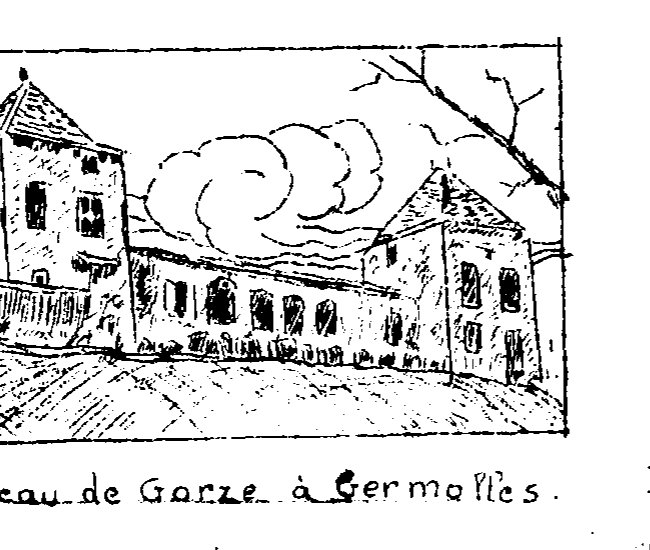
\includegraphics[width=0.45\textwidth]{Illustrations/illus-cures-gorze.png}
\end{figure}

Guillaume Berthet, curé d'Avenas, fonda, par son testament en date du 14 Juin 1622 un Salve Regina, un De Profundis, à la chapelle St-Claude, dans l'église d'Ouroux. Ses héritiers devaient payer annuellement au curé d'Ouroux 10 sols qu'il hypothéqua sur le chènevis situé au dessous du cimetière. Messire Castagne trouvant la rétribution trop faible refusa de dire ces prières. Il convint avec Jean Hugues et Jean Chrysostome Duligier qui possédaient ce chènevis en 1707 de transformer cette fondation et de dire chaque année une messe à la chapelle de St-Claude pour le repos de l'âme du sieur Berthet.

% --- Page imprimée 101 — vue 104
VI - Michel Perrichon nous est également signalé dans le compte de tutelle d'Antoinette Lafond veuve Duligier où nous trouvons : "payée la somme de 5 livres à Messire Michel Perrichon, prêtre vicaire d'Ouroux pour avoir enseigné à lire au fils Duligier, en 1598"

VII - N. Faure était vicaire à Ouroux en Novembre 1615. Il signe comme témoin dans un acte reçu Testenoire notaire royal. Nous le retrouvons encore le 1er Juillet 1626.

VIII - N. Pepide témoin dans le testament de Benoiste de la Palud en Novembre 1622. Un acte également signé par lui porte la date du 7 Avril 1623.

IX - François Jandard, prêtre, vicaire perpétuel est témoin dans l'acte de mariage de Claude Gaze et de Prudence Berthelon. Le contrat est passé à la maison de Lacarelle où résidaient les époux Berthelon, le 1er Février 1622.

X - Benoît Basset, nommé dans un testament fait à Gros-Bois par Toinette Champelly de St-Christophe-la-Montagne au profit de Claudine Viollet, femme Ducroux, le 13 Janvier 1623.

XI - André Litaudon qui était à Ouroux le 2 Juin 1623 et le 17 Juillet 1625 comme le prouvent les actes où il est cité comme témoin.

XII - Philibert Alevesque dont nous retrouvons fréquemment le nom dans les actes notariés du 7 Décembre 1623 jusqu'à la fin de l'année 1625 époque où il fut nommé curé d'Avenas.

XIII - Antoine Cymontel (?). Son nom à peu près illisible se trouve dans le contrat de mariage de Jean du Thel tixier à Ouroux et de Claudine Sauzay, contrat dans lequel il figure comme témoin.

XIV - Jehan Jacquet est témoin dans le mariage de noble Pierre de Boullery sieur de Capital avec Françoise de Peyrieu, le 17 Juillet 1625.

XV - Étienne de La Font. De l'ancienne Famille de la Fonte, plus tard de la Font qui occupa le notariat d'Ouroux jusqu'à la fin du XVIème siècle. Il est nommé vicaire d'Ouroux dans plusieurs actes en 1630 et spécialement dans le contrat de mariage passé au Mas Daguin entre Benoist Métrat et Anne Michou.

% --- Page imprimée 102 — vue 105
XVI-Benoist Morin qui devait plus tard être curé à Émeringes. Son
passage à Ouroux ne nous est signalé que par un seul titre, le tes-
tament de Benoît Gobet "faict en la masure du Thel le vingt hui-
tième jour du moy de décembre l'an mil six cent vingt neuf" où il
signe comme témoin ainsi que Estienne De La Font qui n'est encore
que diacre. Benoist Morin était né à Ouroux où son frère Antoine
exerçait la profession de marchand.

XVII-Rigaud De Maisonneuve prend le titre de curé perpétuel d'Ouroux.
L'expression de curé, employée ici pour la première fois n'est
sans doute qu'une erreur de la part de la rédaction de l'acte. Il
est témoin dans le testament de Suzanne Berthelon femme de Sieur
Aymé De la Font, passé au Château Montagne (Berthu) le 5 Mai 1646.
Nous le retrouvons encore en Mai 1647.

À cette époque Saint Jacques des Arrêts cesse de dépendre d'Ouroux
comme annexe puisque Gilbert Robert et Jacques Arnoux ont le
titre de prêtres vicaires de St-Jacques-des-Arrêts dans le testa -
ment de Claude de Grosbois.

XVIII-Barthélemy Debotton était né à Ouroux en 1650 ou 1652 comme
le prouvent les actes de Baptême de Pierre et de Benoiste Testenoire.
Il nous est resté une pièce curieuse concernant ce curé qui
nous montre la procédure suivie à cette époque pour régler les différends
qui surgissaient entre le pasteur et les fidèles. L'acte
notarié est daté du 16 Juin 1650. Le voici :

"Le jour de la feste du Saint-Sacrement se présentèrent à la
grande porte de l'église Jehan de Chapon escuier, sieur de la Bottière,
St-Julien, commissaire député pour la royale conduite des gens
de guerre passant en ce pays de Beaujolais, principal habitant de
cette paroisse et Pierre de la Font... etc, lesquels s'adressant à
Messire Barthélemy Debitton prêtre, vicaire perpétuel d'Ouroux, lui
remontrent que de toute ancienneté lesdits vicaires perpétuels ont
dit la Passion en ladite église d'Ouroux depuis la Sainte Croix de
May jusqu'à la Sainte Croix de Septembre". Il est probable qu'il
obtempéra immédiatement à un vœu aussi formellement exprimé. Nous
n'avons sur lui aucun autre détail.

% --- Page imprimée 103 — vue 106
XIX - N. Peyras ne nous est connu que par le certificat suivant : "les présentes commissions du roy ont été publiées à mon prosne de grand messe le requérant Messire Testenoyre notaire royal à Ouroux. En foy de quoy j'ai signé : Peyras ". Ce certificat est de 1656.

XX - Jean François Chostard signe dans une cession de droits comme curé d'Ouroux en 1658. Deux de ses paroissiens ayant cherché à différentes reprises de mettre en discussion son honorabilité, Mr Chostard exigea d'eux une rétractation en forme en 1659. En conséquence par acte notorié, les frères Jean et Durand Montel déclarent "qu'ils sont bien marry d'avoir faict querelle et débat avec le dict Messire Chostard et qu'ils le tiennent pour bon ecclésiastique, ne l'ayant jamais reconnu pour aultre ny ouy dire aultrement. Présents : Jean de Chappon escuier, sieur de la Brottière, St-Julien, Rizière et Mr Jean Hugues Testenoire notaire royal".

Nous le trouvons encore comme témoin dans le contrat de mariage de Benoît Trompier de St-Christophe Delle Mélinand passé en la maison seigneuriale d'Arcisse.

Il est le dernier qui ait pris le titre de vicaire perpétuel.

XXI - Jean Chrysostome Morin fut nommé curé d'Ouroux depuis 1664 jusqu'en 1676. Il était frère d'Antoine Morin que nous trouvons fermier des dîmes de MM les chanoines de St-Pierre de Mâcon en 1661 et fermier de la rente noble d'Ouroux et Seigneurie dudit lieu (Alloignet) appartenant à son Altesse royale Dame et Baronne du Beaujolais. Il avait une maison dans le bourg et un petit domaine d'un revenu de 80 livres.

Son père, Antoine Morin fut sans doute le frère de Geoffroy Morin maréchal qui épousa en 1596 Philiberte Testenoire, fille de Jehan Testenoire et de Antoinette De la Font. En 1652 nous trouvons Antoine Morin et Claude Lacondemine comme consuls et leveurs des tailles.

Comme nous l'avons vu plus haut, ce fut sous l'administration de Mr Morin, le 7 Août 1664, que le chapitre St-Pierre de Mâcon céda au curé le tiers des dîmes qui lui appartenaient comme collateur du bénéfice, le chapitre de Beaujeu ayant les deux autres tiers.

% --- Page imprimée 104 — vue 107
Le chapitre refusa-t-il d'admettre cet arrangement ou bien voulut-il profiter de l'occasion qui lui était offerte d'empiéter sur les droits du curé ? Le fait est que Mr Morin intente un procès contre M les Doyen, Chanoines et Chapitre de Notre Dame de Beaujeu qui avait usurpé une partie des revenus de la cure. Ce procès commencé en janvier 1667 se termina le 22 Novembre de la même année par une transaction. Mr Morin transmit au chapitre le tiers des dîmes qui lui appartenait et le Chapitre s'engagea à lui fournir la portion congrue.

À la fin de l'année 1670 et au commencement de l'année suivante, les difficultés surgirent de nouveau entre le curé d'Ouroux et le Chapitre de Beaujeu. Il était urgent de faire des réparations au clocher et au chœur de l'église et c'était au Chapitre à subvenir à la dépense. Il refusait tout en en constatant la nécessité. Mr Morin le fit assigner à deux reprises différentes donnant chaque fois 10 sols au lieutenant général pour faire saisir.

Mr Morin, pendant son séjour à la cure d'Ouroux donna fréquemment des preuves de son zèle pour le culte et l'embellissement du sanctuaire. Il mit ordre aux fondations anciennes, exigeant des héritiers les preuves de leurs droits, ne craignant pas pour mettre fin aux abus qui s'étaient introduits, d'entreprendre des procès longs et coûteux. Et cependant, bien loin d'être opposé à ces fondations pieuses il les encourageait lui-même comme nous le prouvent les titres qui nous ont été conservés et que nous relaterons en leur lieu.

Néanmoins les intérêts matériels de la paroisse n'absorbèrent pas tellement l'activité de Mr Morin qu'il ne chercha à faire prospérer également ses intérêts spirituels. Dès les premières années de son ministère paroissial il se proposa de restaurer la confrérie du Très Saint-Sacrement dans la paroisse. Cette confrérie y était instituée depuis longtemps, mais par suite du malheur des temps, elle avait été complètement abandonnée. Il fut, du reste, admirablement secondé par les principales familles De Gorze, de la Font et Duligier Testenoire.

La première élection des dignitaires de la confrérie eut lieu le 5 Août 1668 dans l'église, après le chant du Veni-Creator ; avant de se séparer on chanta le Te Deum en action de grâces. Ces élections paraissent avoir eu lieu tous les deux ans. Dans la première et dans
% --- Page imprimée 105 — vue 108 (suite)
la seconde nous trouvons comme conseillère Demoyselle Catherine Alacoque, femme de Antoine de la Font bourgeois d'Ouroux et parente de la bienheureuse Marguerite Marie.

En 1676 Mr Morin quitta Ouroux pour aller curé à Emeringes. Il succéda à son oncle Benoit Morin que nous avons vu à Ouroux en 1629 vicaire perpétuel. Dès l'année 1664 Mr Morin quitta Ouroux, nous le trouvons désigné comme Chapelain de la chapelle Notre Dame de Pityé dans l'église de cette paroisse. Par contrat du 21 Octobre de cette année il vendait à Guillaume Gailleton vigneron de Fleurye une vigne sur Lancié, au lieu appelé Perrichon, contenant trois ouvrées d'homme, moyennant 200 livres tournois et 11 livres d'étrennes. Le dict acquéreur s'engageait à payer chaque année 6 deniers tournois aux chapelains de la dite chapelle.

Par acte reçu Testenoire, le 4ème jour de Février 1679, Mr Morin Benoit, précédemment curé à Emeringes et Jean Chrysostome Morin, actuellement curé de la paroisse, fondèrent 12 messes dans leur chapelle dédiée à St-Joseph qu'ils avaient fait construire dans l'église d'Emeringes et dont ils réservèrent le droit de patronage à leurs héritiers. Étant curé, Benoit Morin avait fait construire de ses propres deniers une tour carrée, au côté droit du chœur avec un tombeau pour lui et ses successeurs. Comme il n'y avait pas de clocher à l'église, il fit élever cette construction à une hauteur suffisante et y fit placer les cloches.

Monsieur Morin, devenu curé d'Emeringes, conserva néanmoins toujours des rapports avec son ancienne paroisse. Nous le voyons en 1683 opérer encore le règlement des comptes de l'église et de la confrérie du St-Sacrement à Ouroux. Son neveu Antoine Morin dont il avait été le tuteur étant fermier, dans la période qui s'étend de 1697 à 1702, de la rente noble d'Ouroux appartenant à son Altesse royale, Monsieur Baron de Beaujolais parvenait difficilement à recouvrer les sommes qui lui étaient dues. Il avait alors recours à son oncle, Mr le curé d'Emeringes ; aussi celui-ci écrivait-il à Mr Duligier son fondé de pouvoirs, le 26 février 1699 ; je vous supplie de faire payer les débiteurs de la rente d'Ouroux. J'ai adressé quatre vingt quatorze éscus pour les deux dernières années. Je serais bien aise d'en retirer ce qu'on pourra". En d'autres termes il avait à
% --- Page imprimée 106 — vue 109 (suite)
peu près tout payé, puisque vingt ans auparavant la rente ne s'élevait qu'à 110 livres.

En 1708 les mêmes difficultés recommencèrent. La misère était extrême. On se mit en mesure de faire saisir tous les fermiers de Lacarelle. Mr Morin qui, à cette époque, était à Lyon, écrivit immédiatement à Mr Duligier, notaire à Ouroux, et qui était sans doute fermier de la même rente, cette lettre si digne d'un pasteur :

"Je vous prie de ne pas faire saisir sur les fermiers de Lacarelle suivant la sentence que vous avez fait signifier à Madame de Vertpré qui m'est venue trouver, les larmes aux yeux, disant que les fermiers n'ont rien, pas même de quoi vivre et que vous n'avancerez rien autre que Monsieur de Lacarelle en serait très fâché ; auquel je parlerai si fortement que je l'obligerai ou je ne pourray, par mes raisons, non seulement à payer le contenu en l'obligation, mais encore les arrérages du passé. 16 juin 1708 ;"

Monsieur Jean Chrysostome Morin mourut probablement à Lyon, chez Antoine son neveu qui y résidait. Cette lettre est la dernière qui porte sa signature.

XXII-Claude Corteille succéda à Mr Morin et fut curé d'Ouroux de 1676 à 1679. Il fut installé par Chrysostome Morin le 18 Janvier 1676. L'acte d'installation porte qu'il était "prestre du diocèse de Lion et aultres lieux". Il avait obtenu ses lettres de provision de N.S.P. le Pape Clément X. Monsieur Morin, au moment même de la prise de possession se réserve formellement une pension dont le taux n'est pas spécifié sur ledit bénéfice cure. Claude Corteille n'était, pour ainsi dire, qu'un auxiliaire et Mr Morin conservait le titre de curé proprement dit.

XXIII-Elzéar Berthet né en 1641 fut curé de St Barthélemy d'Ouroux du 11 novembre 1680 au 14 août 1701. Appartenait-il à l'illustre famille des Berthet de Gorze ? Cela est probable ; néanmoins aucun document ne nous permet de fixer sa généalogie. La famille de Gorze possédait à Ouroux une chapelle et d'assez belles terres ; il est possible que Mr Morin qui, lui, était natif de cette paroisse et conservait toujours des rapports d'intérêt et d'affection avec Ouroux ait sollicité la nomination de Elzéar Berthet.

% --- Page imprimée 107 — vue 110
En 1683 nous le voyons acheter un tabernacle fourni par Mr Novil maître sculpteur à Lyon demeurant devant le grand collège, au prix de 120 livres. Il remplaça sans doute le tabernacle en bois sculpté dont la porte existe encore à la cure et qui rappelle, par ses ornements, l'époque de la renaissance. Nous trouvons également mentionné l'achat "des figures de St-Antoine et de St-Barthélemy"

La même année Mr Berthet voulant faire construire une sacristie plus spacieuse à côté du maître-autel, n'ayant du reste dans sa fabrique aucune ressource, fit appel à la générosité des principaux Seigneurs de la paroisse. L'énumération de ses divers dons nous fournit l'occasion de faire connaître la situation des bienfaiteurs de cette époque.

Le Chapitre de Beaujeu donna.....20 livres
Le Seigneur de Barmondière.......21    -
Le Seigneur de Gorze.............1     -
Le sieur Dubost La Blanche.......12    -
Mr Morin curé d'Emeringes........1     -
Mr d'Avenas......................5     -    10 sols
Jean Chrysostome de Grosbois.....5     -
Sr Lieutenant d'Aigueperse:......3     -
Mre Antoine Dubost...............5     -
Madame de Rizières...............1     -

Enfin Jean Chrysostôme de Grosbois fournit le bois nécessaire pour le couvert.

Mr Berthet mourut à la suite d'une courte maladie "muni de tous les sacrements, après avoir gouverné la paroisse d'Ouroux avec tous les soins et toute la vigilance possible pendant 22 ans, le 13 Août 1701 et fut inhumé dans le tombeau destiné aux prêtres dans l'église, le 14 Août par Messire Claude Chastellet curé de St-Jacques-des-Arrêts, assisté des vénérables curés de Germolles, St-Mamert, Avenas et Trades.

Mr le curé de St-Jacques administra la paroisse jusqu'au milieu de septembre de la même année, époque où fut nommé :

XXIV-Jean Castagne qui naquit en 1665 et fut curé d'Ouroux pendant 20 ans, du 14 ou 15 septembre 1701 jusqu'au 10 février 1721. Il accepta en 1707 la fondation faite par Jean Hugues et Jean Chrysostôme Testenoire dans leur chapelle comme nous le verrons, et reçut à cet effet le pré appelé Chenevis situé près de la cure, entre l'ancien cimetière et la rivière.

% --- Page imprimée 108 — vue 111
Rien de bien remarquable, à part la famine, ne signale le passage de Mr Castagne à Ouroux. Au mois de Janvier il tomba malade. M. Castellat, curé de St-Jacques, vient le remplacer, puis Mr de Grosbois qui s'était retiré dans sa famille. Mr Castagne mourut le 20 février 1721 et fut enterré dans l'église d'Ouroux au tombeau de ses prédécesseurs.

Nous venons de prononcer le mot de famine, nous devons ajouter celui d'épidémie, fléaux qui désolèrent nos régions du Beaujolais, et, en particulier, notre paroisse d'Ouroux. L'année 1709 fut en effet "l'année chère, l'année cruelle". Ces fléaux confondus au milieu de tant d'autres calamités qui écrasaient le peuple ont laissé cependant peu de souvenirs parmi nous. Les contemporains ne nous ont laissé sur ce sujet aucun détail, mais les chiffres, du moins, dans les registres mortuaires parlent avec une terrible éloquence.

"L'hiver de l'année 1709 fut, dans toute la France, d'une rigueur sans exemple. Le pays était écrasé par de grands désastres militaires et par l'excès des impôts. Cette calamité nouvelle mit le comble à la misère publique, engendra la famine suivie de maladies épidémiques et occasionna une énorme mortalité"

"Le froid intense qui sévit du 6 février au 23 février gela la Saône et même le Rhône à une profondeur si considérable que la glace portait les plus lourds chariots. Ce froid excessif fit périr les noyers, les châtaigniers, une grande partie des vignes et toutes les semailles.

"L'année 1708 n'avait donné qu'une demi récolte. La récolte de 1709 se trouvait anéantie. Aux gelées destructives de l'hiver succédèrent des pluies sans fin et il survint une famine telle qu'on n'en avait pas vu depuis 1573.

"Le prix du pain à Villefranche est de 3 sols 6 deniers la livre

Nous avons trouvé dans un registre de la famille Duligier Testenoire le prix du seigle pendant les années qui précédèrent et qui suivirent cette année néfaste. On sait d'ailleurs que le froment était rare dans nos montagnes et que le seigle formait la nourriture exclusive de nos populations. Voici donc quels furent ces prix :
En 1705 - 1706 - 1707 - 1708 - 1709 - 1710 - 1711 - 1712 - 1713
17 sols   15s    15s    2"5s   3"9s   1"10s  1"30s  2"     3"

% --- Page imprimée 109 — vue 112
On voit d'après ce tableau la différence considérable entre le prix du seigle en 1705 et en 1709. L'augmentation se dessine déjà d'une manière grave en 1708 ; elle est le résultat de la demi-récolte signalée plus haut. En 1710 les prix sont peu exagérés au-dessus de leur cours normal pour remonter ensuite en 1713. Et cette différence s'explique assez naturellement.

À l'époque où la famine sévissait dans toute son intensité en 1709, la récolte étant absolument nulle, les autorités prirent des mesures pour approvisionner les marchés, organiser des transports de vivres. De là, la baisse considérable qui se manifesta en 1710. Mais ces mesures extraordinaires ne pouvaient devenir la règle générale ; les provisions s'épuisent et les prix augmentent de nouveau d'une façon inquiétante.

D'ailleurs point de secours organisé dans nos paroisses. Les impôts excessivement onéreux à la suite des guerres malheureuses que Louis XIV faisait en Espagne enlevaient à nos populations toute possibilité de soustraire aux fléaux qui les décimaient. Nous avons vu Mr Duligier fermier de la rente noble d'Ouroux faire saisir tous les fermiers de Lacarelle. Comment pouvaient-ils, dans ces conditions, se procurer le pain nécessaire à leur subsistance et à celle de leurs familles ?

En 1701, on donnait à un homme 4 sous par jour pour sa subsistance. On comprend facilement que le prix du pain en 1709 était inabordable pour le plus grand nombre. Aussi on arrive bien vite aux expédients. Les anciens, à la fin du siècle dernier, se souvenaient parfaitement d'avoir entendu dire à leurs ancêtres qu'à une époque qu'ils ne savaient pas préciser, mais qui est bien celle qui nous occupe, on faisait sécher les racines de fougères que l'on réduisait en poudre et dont on faisait ensuite du pain. On sait que la pomme de terre ne fut introduite qu'à la fin du siècle dans notre région.

Déjà en 1694 et 1698 le prix du seigle s'était élevé à Ouroux à 4"10 sols et celui de froment à 5" ce qui faisait à peu près 30 fr en 1880, la mesure. Ajoutez à cela que nos contrées subissaient tous les effets d'une guerre désastreuse : anéantissement du commerce, impôts excessifs, mesures financières ruineuses, création d'offices
% --- Page imprimée 110 — vue 113 (suite)
inutiles et vexatoires, insuffisance répétée des récoltes; il sera facile de comprendre combien il était difficile de subvenir à toutes les difficultés inhérentes à une famine aussi générale que le fut celle de 1709.

Peu après le début de la famine survint une maladie épidémique, "une espèce de peste" qui causa une grande mortalité dans notre paroisse comme d'ailleurs dans toute notre région.

En dépouillant les registres mortuaires des huit années qui précèdent l'épidémie, c'est-à-dire de 1700 à 1708 inclusivement, on trouve que la mortalité annuelle oscille entre 10 et 15, une moyenne de 1 décès par mois. Une seule fois en 1708 le nombre des décès s'élève à 16, mais l'année 1700 n'en offre exceptionnellement que 6. Nous pouvons, du reste, admettre, je crois, une population approximative de 900 à 1000 habitants, le nombre des naissances ayant été en moyenne de 22 pendant les trente dernières années. Nous allons voir maintenant ce que devient cette population par suite de l'épidémie.

Les trois premiers mois de l'année 1709, la proportion demeure normale. On trouve en janvier un décès; en février, deux; en mars deux également. Le mois d'avril en offre quatre; jusque là rien que de très ordinaire; mais au mois de mai on reconnaît l'action non douteuse de l'épidémie. La mortalité monte à neuf. Elle s'élève à dix au mois de juin, à quatorze en juillet, puis elle redescend sensiblement les mois suivants, à huit en Août, septembre, octobre et novembre; à cinq au mois de décembre.

En janvier 1710 la mortalité reprend une nouvelle recrudescence il y a onze décès, sept en février; mars en présente deux seulement ; mais en avril nous en retrouvons sept. À cette époque l'épidémie paraît éteinte; les mois suivants ne présentent en moyenne que un ou deux décès.

Du 1er avril 1709 au 13 septembre 1710 c'est-à-dire en 16 mois, il y eut cent huit décès. Sur ce nombre nous en trouvons plusieurs qui moururent dans les champs; quatre pauvres étrangers qui imploraient la charité des habitants d'Ouroux; malgré les ordonnances, en vertu desquelles chaque paroisse était obligée de nourrir ses indigents, furent trouvés morts d'inanition dans les granges qu'on leur avait offertes comme abri.

% --- Page imprimée 111 — vue 114
Si nous étudions l'âge des personnes décédées, nous constatons que les enfants et les vieillards ont été presque exclusivement atteints. Nous en trouvons 44 en dessous de 10 ans, 14 au-dessus de 60 et 3 seulement de 20 à 30 ans. Ces chiffres semblent prouver que la faim et les privations, plus difficiles à supporter par le tempérament délicat des enfants et des vieillards ont dû faire un plus grand nombre de victimes que l'épidémie elle-même.

Tels sont les quelques détails intéressants à conserver sur une période que l'on peut regarder comme la plus néfaste de toute notre histoire. Durant ces jours d'épreuve Mr Castagne fut toujours à son poste. Sa comptabilité n'ayant pas été tenue en règle pendant ces années de misère, par suite sans doute de ses nombreuses occupations, il est impossible de connaître quelles furent les mesures prises par lui pour aider les malheureux à résister aux fléaux.

XXV-N... Perrachon fut curé du 28 février 1721 jusqu'au 25 novembre 1732. Rien de particulier à signaler sur son administration ; il ne nous est d'ailleurs connu que par les registres de catholicité. Il n'est pas mort à Ouroux ; c'est lui, sans doute, que nous retrouvons à Chiroubles en 1680.

Claude de Gros-Bois de concert avec Mr Brochard, vicaire de la paroisse administra Ouroux jusqu'à l'arrivée de

XXVI-Antoine Guillin du Montet né à St Bonnet des Bruyères, le 8 janvier 1702, fut baptisé le lendemain et eut pour parrain Messire Antoine Moiroux, prêtre et chanoine en l'église d'Aigueperse et pour marraine Damoiselle Claudine de Nivière, femme de Messire Philibert de Laplace, notaire royal et procureur en la ville de Beaujeu. Il fut tenu sur les Fonts Baptismaux par Jean, son frère.

Mr Guillin fut nommé à la cure d'Ouroux le 27 octobre 1733

Il était fils de Denis II Guichard Guillin du Montet, sieur de Montet, fief situé en la paroisse de St Bonnet des Bruyères, juge de la Châtellenie de Chevagny de Lombard (1696), même paroisse, notaire royal au dit Chevagny (1713-1730) et de Elisabeth de la Font de Pougelon. De treize enfants issus de ce mariage, Antoine fut le neuvième.

Il n'entre pas dans mon plan de faire ici l'histoire de la famille de Guillin qui remonte jusqu'au milieu du XIVe siècle. Qu'il me
% --- Page imprimée 112 — vue 115 (suite)
suffise de dire qu'elle contracta des alliances avec les familles les plus célèbres de nos contrées. Elle posséda pendant trois siècles, les fiefs de : Le Montet, Les Guillin, Chevagny, le Lombard, La Roche, Les Cloux, Pougelon, Le Sauzey, Avenas ; celui de Poleymieu lui appartint également.

Les armes de cette famille étaient : Coupé d'argent et de sable, au lion d'or brochant sur le tout ; support : deux aigles éployés d'or.

Un de ses oncles paternels Jean Antoine de Guillin du Montet, docteur en Théologie, fut chanoine doyen d'Aigueperse et à ce titre curé de St-Bonnet des Bruyères.

Deux de ses neveux méritent une mention particulière. Son frère François Gabriel né en 1700 eut de son mariage avec Françoise Marie Perrin, cinq enfants dont deux surtout ont laissé dans l'histoire de glorieux souvenirs.

L'aîné, Antoine Guillin du Montet, seigneur de Pougelon, Les Cloux, le Sauzey, Avenas était probablement le filleul de son oncle, curé d'Ouroux. Celui-ci détermina son neveu à acheter le château et le fief du Sauzey et Avenas le 5 août 1778. Il fut successivement avocat au parlement et Cour de Lyon (1754), bâtonnier de l'ordre des avocats, recteur et administrateur des hospices et Grand-Hôtel-Dieu de Lyon (1769-1770), puis premier officier du Comte de Lyon, juge général et civil de police, gruerie et voirie pour la ville et le Comté, juge particulier, et outre, de vingt-huit paroisses (Anse, Belleville, Rive de Giers, Vaugneray, Ste-Foy-les-Lyon, etc.)

Exilé à Valfleury, sous Louis XVI, pour avoir défendu les privilèges de Lyon, il rentra bientôt triomphalement dans cette ville.

Homme impassible et d'une grande énergie à qui le roi songea pour la succession de Necker, qui n'hésita pas à sacrifier sa popularité pour défendre l'ordre au péril de ses jours et qui devint, par la force des choses, le chef le plus influent du parti du roi à Lyon. Il fut arrêté comme tel (4 décembre 1790), transféré à l'Abbaye de Paris, les fers aux mains, puis mis en liberté (octobre 1791) par traité et convention spéciale du roi lorsque celui-ci accepta la Constitution.

Retiré à Nantes avec sa femme et ses filles (1791-1793) il fut arrêté de nouveau (1793) et enfermé dans la prison de cette ville d'où
% --- Page imprimée 113 — vue 116 (suite)
il devait être expédié à Paris. Mais il fut sauvé par le dévouement
intéressé du geôlier. Mis en liberté après la mort de Robespierre, il
mourut au château de Pougelon le 17 Août 1817.
    Son frère, Marie Aimé Guillin du Montet, sieur de Poleymieu, chevalier
des ordres du roi, capitaine de vaisseau et chef d'escadre, gouverneur
lieutenant général du Sénégal, rivière de Gambie et des possessions
françaises (1765-1785) naquit à Lyon le 2 Mai 1730 et fut massacré
à Poleymieu le 26 Juin 1791.
    Entré très jeune dans la marine, il fut fait chevalier de St-Louis
à 16 ans pour action d'éclat. Dans un combat, il se précipita à la
mer avec un baril de poudre enflammée dont l'explosion eut pu faire
sauter le navire.
    Il servit d'abord sur les navires corsaires du Marquis de Roux ;
fut ensuite lieutenant de la flotte de la Compagnie des Indes, entra
à 29 ans dans la marine royale et se signala par ses exploits dans
la guerre contre les Anglais. Il exerça le commandement en Afrique
pendant vingt ans avec autant de capacité que de zèle et de fermeté
    Il se retira (1786) âgé de 56 ans avec 28 mille livres de pension
militaire et acheta le château et la terre de Poleymieu sur la montagne
de Limonest.
    Son arrivée à Poleymieu fut l'occasion de grandes réjouissances.
On se plaisait à rappeler les hauts faits d'armes de cet homme sur
lequel on fondait les plus heureuses espérances. Dans une chanson,
composée à cette occasion, on proclame surtout ses vertus guerrières
Nous relevons les passages suivants :
    I-Ce guerrier qui s'avance
      A le plus grand renom
      Cet illustre marin
      Compagnon de d'Estaing
      Émule de Suffren
    II-Dans les deux hémisphères
      Il vainquit pour nos rois
    III-Guillin aux champs de Mars
      courut plus de hasards
      Qu'Alexandre et César
    VII-Son frère nous présage
      La paix et le bonheur
      C'est la vivante image
      D'un bon législateur
    Un tel enthousiasme était loin de présager les faits douloureux
% --- Page imprimée 114 — vue 117 (suite)
qui ne devaient pas tarder à se produire.

Bientôt, en effet, il fut désigné aux soupçons et aux fureurs populaires, comme frère d'Antoine Guillin de Pougelon, chef du parti royaliste à Lyon et qui venait d'être arrêté. Des perquisitions répétées et vexatoires furent exécutées chez lui pour y rechercher les armes destinées aux royalistes. Le 26 Juin 1791, peu après la fuite et l'arrestation du roi Louis XVI, les passions révolutionnaires étant de nouveau surexcitées, il se vit attaqué dans son château par une foule de plus de cinq mille personnes armées où figuraient les bandes des faubourgs de Lyon, au milieu des habitants des paroisses de Quincieux, Chasselay, Poleymieux et autres, venus pour piller et brûler.

Après un semblant de résistance, Mr Guillin ayant ouvert pour parlementer, il fut saisi, massacré, dépecé par un garçon boucher ; sa tête fut promenée au bout d'une pique, ses membres partagés. Des cannibales firent apprêter et mangèrent dans une auberge de Neuville-sur-Saône son cœur et une partie de ses chairs palpitantes.

Mais revenons au sujet qui nous occupe. Mr Guillin du Montet, avons-nous dit, avait été nommé curé d'Ouroux le 27 Octobre 1733.

Les curés, jusqu'à lui, sans fortune personnelle, ne trouvant d'ailleurs que des ressources très restreintes dans la paroisse, obligés souvent de recourir à la justice pour obtenir du Chapitre de Beaujeu les réparations nécessaires à l'église, l'avaient laissée dans un délabrement complet. Les désastres causés par les armées protestantes et par les troupes de la Ligue vers 1590 n'avaient même probablement jamais été réparés. Mr Guillin se mit immédiatement à l'œuvre, et, durant les quarante années qu'il dirigea cette paroisse, on peut dire, qu'il n'eut qu'un seul but : donner au culte religieux toute la splendeur possible.

Et pour cela il s'imposa fréquemment des sacrifices personnels considérables pour embellir l'église, se procurer des ornements convenables et souvent d'un grand prix. Le détail de ces diverses acquisitions est d'ailleurs assez intéressant par lui-même pour que je m'y arrête quelques instants. On verra par là même quel était l'ameublement de notre église au milieu du XVIIIème siècle.

% --- Page imprimée 115 — vue 118
Dès son arrivée à Ouroux (1734) il fit donner une mission qui fut prêchée par les Révérends Pères Edmond d'Arnay le Duc et Silvestre de Saulieu, Capucins missionnaires apostoliques. Une croix élevée près de l'église fut destinée à en rappeler le souvenir.

La même année il fit refaire le beffroi par François Bellandin de Jullié, moyennant le prix de 100 francs ; il y avait déjà à cette époque quatre cloches. Plus tard en 1766 il faisait refondre et augmenter à ses frais la grosse cloche et la troisième par Baret fondeur à Mâcon. On ne prenait que deux livres pour les conduire d'Ouroux à la Grange du Bois. Plus tard, en 1773, Mr de La roche Lacarelle donnait l'arbre avec lequel on a fait la montée du clocher qui existe encore à cette heure. Ajoutons à toutes ces dépenses extérieures celles exigées par les réparations du cimetière qui incombaient à cette époque à la Fabrique.

L'intérieur de l'église fut plus spécialement l'objet de la sollicitude de Mr de Guillin. Il fit construire des bancs plus convenables et plus commodes pour les fidèles (1736-1754) ; boiser la chapelle de Notre Dame (1738), le chœur et la chapelle de St Barthélemy (1754) ; la nef de l'église (1758) ; reconstruisit la sacristie (1752). Il remplaça le grand bénitier par celui qui existe encore aujourd'hui. Il est en marbre de Tramayes et a coûté quinze livres. La table de communion actuelle fut achetée par son successeur en 1779 et fournie par Bourgeot, serrurier à Villefranche.

L'église d'Ouroux, trop petite pour la population ne comprenait, pour ainsi dire, que la nef (voir le plan, plus loin). Trois chapelles seigneuriales en occupaient la majeure partie. Mr Guillin résolut d'utiliser l'espace qui était à sa disposition et fit prolonger les deux nefs latérales. Pour cela il n'eut qu'à construire une chapelle du côté de l'Évangile et deux du côté de l'Épître. Il y avait, dès lors, neuf autels avec leurs pierres sacrées (1754).

À son arrivée à Ouroux il trouva dans l'église les tableaux de la Ste Vierge, de St-Barthélemy, St-Claude et Ste Catherine. Il en acheta six autres à Mâcon au prix de 144 livres (1759) ; il en avait déjà placé un aux Fonts Baptismaux, représentant le Baptême de Notre Seigneur (1754) qui fut remplacé par un autre reproduisant le même sujet (1759).

% --- Page imprimée 116 — vue 119
Enfin en 1767 il se procura ceux de la Sainte Famille et de l'Ange Gardien au prix de 36 livres et de St-François de Sales au prix de trente livres.

Mêmes dépenses en fait de statues. Il n'y en eut qu'une dans le principe : celle de Notre Dame de Gré ou de Grez. Est-ce la statue actuelle de la Sainte Vierge qui paraît ancienne ou bien celle de Notre Dame de pitié de Michel Ange ? Je l'ignore. Nous avons vu ensuite Mr Elzéar Berthet achetant "les figures de St-Antoine et de St Barthélemy". Mr Guillin en 1752 remplaça ces deux dernières par d'autres statues des mêmes saints mais plus grandes et plus dignes des patrons de la paroisse. Plus tard (1765), il acheta une nouvelle statue de la Sainte Vierge puis une autre de Saint Louis et de St Joseph. Ces deux dernières furent placées aux deux côtés du Maître-Autel. Celle de la Sainte Vierge représentait Marie tenant entre ses deux bras le corps inanimé de son divin fils ; elle existe encore à cette heure. Enfin en 1776 il acheta 6 autres statues dont les sujets nous sont inconnus, au prix de 576 livres.

\begin{figure}[ht]\centering
    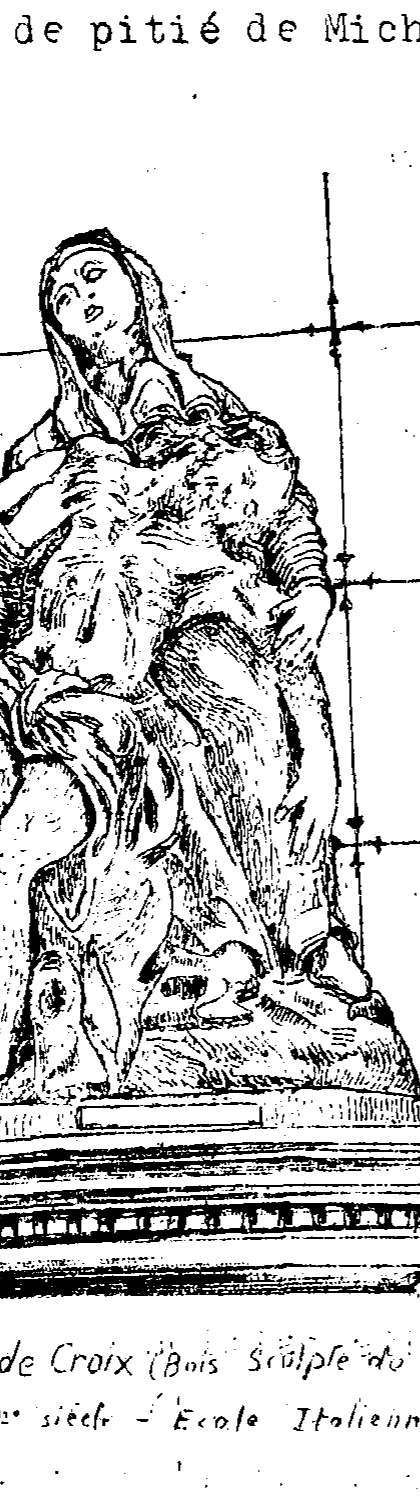
\includegraphics[width=0.24\textwidth]{Illustrations/illus-cures-descente-croix.png}
\end{figure}

D'après un inventaire de 1819, fait par Mr Polloce, il y avait dans l'église d'Ouroux 9 statues "presque hors de service" et 18 tableaux "très vieux". Ces statues et ces tableaux n'étaient sans doute pas des chefs d'œuvre ; il est regrettable néanmoins qu'on les ait fait disparaître ; il eût été facile de les conserver au presbytère.

Rien de surprenant de voir Mr Guillin consacrer les ressources de sa paroisse à l'achat de tableaux et de statues ; c'était un usage
% --- Page imprimée 117 — vue 120 (suite)
général à cette époque, usage qui entrait parfaitement dans les vues de l'église. Les évêques n'avaient-ils pas inséré dans les catéchismes mis entre les mains des enfants cette demande : Que faut il faire pendant les offices ? Et la réponse était : il faut regarder les images ! Et en effet, l'immense majorité des fidèles ne savait pas lire. Et alors on fixait les imaginations par la vue des vitraux, des tableaux, des statues qui étaient pour l'intelligence et pour le cœur, une véritable prédication. Les fidèles s'attachèrent, involontairement, à ces statues, à ces tableaux devant lesquels ils se sont agenouillés dans leur enfance et c'est toujours pour eux un sujet de tristesse de les voir disparaître.

Je me contenterai de donner une rapide énumération des dépenses que fit Mr Guillin en ornements et en vases sacrés. Il acheta un encensoir et sa navette, des burettes et leur plateau, le tout en argent au prix de cinq cents livres ; des chandeliers en argent au prix de 1321 livres et un crucifix du même métal précieux à la confection duquel on employa pour 366 livres d'argent. Enfin 2 nouveaux chandeliers d'argent exigèrent une dépense de 634 livres. Dès son arrivée à Ouroux il avait fait réargenter quatre lampes et en avait acheté trois autres. Il prescrivit de tenir allumées pendant les offices celles de St-Antoine et de St Barthélemy. Plus probablement il ne fit que remettre en vigueur un ancien usage tombé en désuétude.

Mr Guillin, on le voit, fit des dépenses considérables pour doter son église, non seulement de ce qui était nécessaire et utile au culte mais encore pour lui donner un luxe qui devait être rare dans nos paroisses de campagne. Malheureusement tous ces objets précieux ne devaient subsister que quelques années à peine, puisque la Grande Révolution était appelée à renouveler parmi nous les actes de vandalisme et de vol dont on avait déjà été témoin à l'époque de l'invasion des Protestants.

L'ancienne horloge dont la disparition, il y a une quarantaine d'années, a été si vivement regrettée de l'ensemble de la population d'Ouroux, avait été également achetée par Mr Guillin en 1754. Elle lui fut vendue par Jean Fournier, horloger, à Morbière (Comté) au

% --- Page imprimée 118 — vue 121
\begin{figure}[ht]\centering
    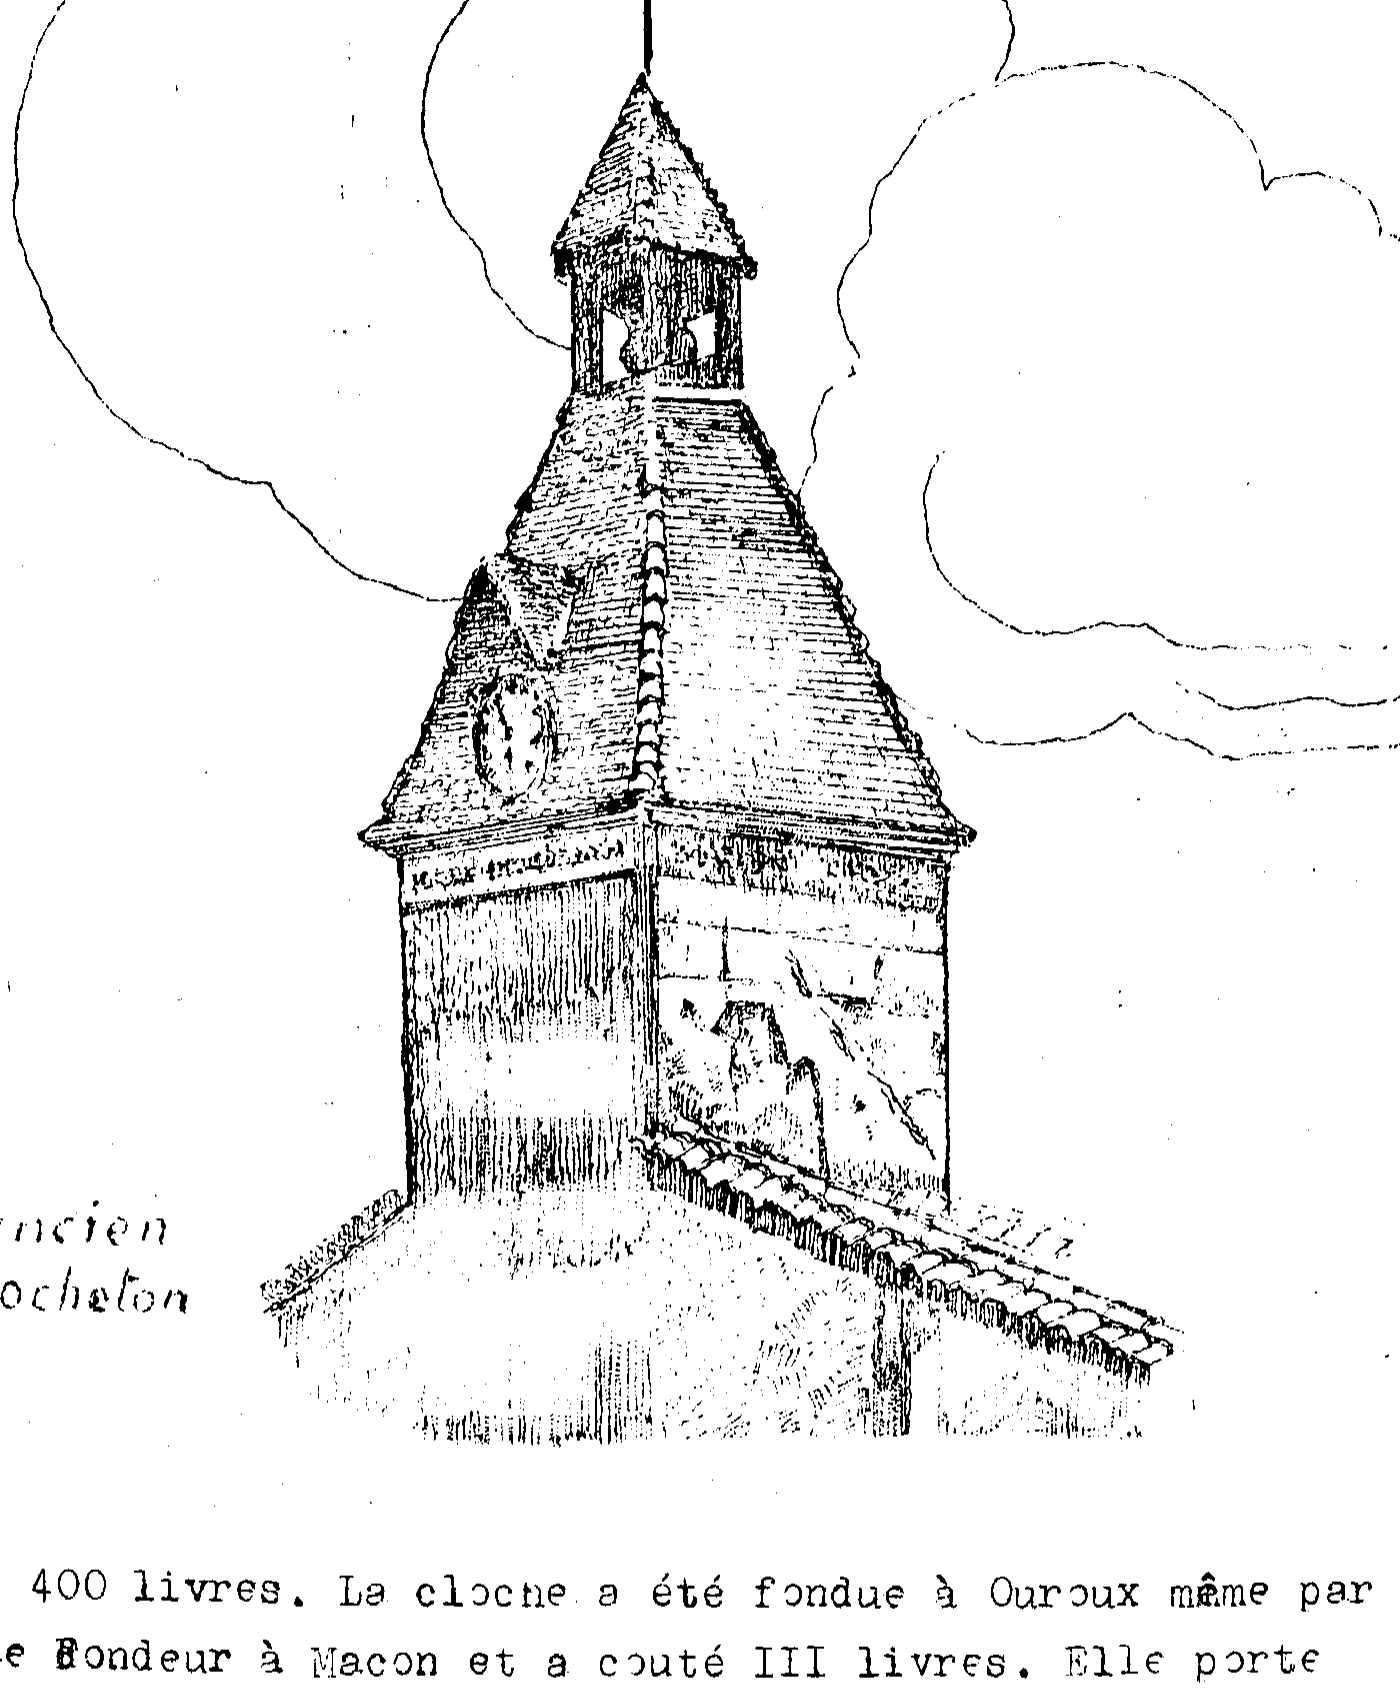
\includegraphics[width=0.48\textwidth]{Illustrations/illus-cures-clocheton.png}
\end{figure}

prix de 400 livres. La cloche a été fondue à Ouroux même par Arnaud Laplatte Fondeur à Mâcon et a coûté 111 livres. Elle porte cette inscription :
	La mort est certaine
	Le jour est incertain
	L'heure encore plus. 1754
	Laplatte de Mâcon m'a fait

	On construisit pour recevoir cette horloge une tour carrée surmontée d'un campanile dans lequel fut placée la cloche. S'inspirant des inscriptions de celle-ci on reproduisit au sommet de la tour ces deux inscriptions : "Je sonne ma dernière heure" et "c'est l'heure d'aimer Dieu"

	En 1830 Mr Polloce fit transporter le campanile sur la grande porte de l'église et la tour disparut.

% --- Page imprimée 119 — vue 122
Le zèle de Mr Guillin ne se borna pas, comme on pourrait le croire en lisant plus haut la liste de ses nombreuses acquisitions à l'ornementation de l'église. Sa sollicitude s'étendit à tout ce qui pouvait intéresser l'avenir de la paroisse. Nous verrons, dans un chapitre spécial, tout ce qu'il fit pour l'instruction des enfants, l'établissement d'une maison d'école à ses frais, la fondation d'une rente au profit de la Fabrique et des pauvres. À ce dernier titre, c'est à lui qu'on doit ici l'établissement de l'institution si utile du Bureau de Bienfaisance.

En 1774 il sollicita un secours particulier de Mr le Duc d'Orléans pour les pauvres d'Ouroux ; il en obtint une somme de 50 francs

Je ne saurais passer sous silence la fondation d'un lit à l'hôpital de Beaujeu par acte passé le mercredi 2 Janvier 1754 et pour lequel il donna de ses propres deniers la somme considérable à cette époque de 3000 livres. Il acquit également de Messire Michel Comte de Fautrière seigneur de Corchevas, Montolieu... et autres lieux, un bois appelé Chastelet au prix de 500 livres. L'acte de vente porte une condition qui est la preuve la plus frappante du zèle de ce saint prêtre. Lui et ses successeurs curés d'Ouroux en jouiront en vrais propriétaires à la charge d'entendre en confession les enfants non communiants deux fois dans le cours de chaque année. Les successeurs pourront couper les arbres, les faire descier pourvu que les ais soient employés aux réparations de la nef, des chapelles et de la sacristie. Les menus bois appartiennent au curé.

Ce bois, au moment de l'achat, n'était composé que de quelques chênes et sapins. Les successeurs de Mr Guillin comprenant qu'il y aurait là et dans un avenir prochain une ressource considérable pour la Fabrique, en prirent un soin tout particulier. Et les anciens se rappelaient encore Mr Polloce vêtu d'une mauvaise soutane, portant lui-même son modeste dîner et travaillant à entourer le bois d'un mur qui existe encore. L'ouragan qui fit de si grands ravages dans notre région le 21 février 1879 laissa à peine une dizaine de sapins debout. Ceux qui furent renversés avaient de 80 à 90 ans.

Le zèle du pasteur porta ses fruits. Il serait facile de trouver de nombreuses preuves de la piété de notre population à cette époque. Je ne veux en choisir qu'un exemple pour bien montrer la foi de
% --- Page imprimée 120 — vue 123 (suite)
nos pères.

Les fidèles se faisaient un honneur et un devoir de prendre une part active aux exercices du culte et leur empressement à s'offrir pour porter les insignes religieux et aider le prêtre à l'autel devint tellement général qu'il fallut mettre ces fonctions aux enchères. Elles avaient lieu publiquement, le jour de l'Ascension. Je prends au hasard l'année 1736.
La bannière fut adjugée... 25 sols
La croix - - - - 1 livre
Le cierge pascal - - 16 sols
L'encensoir - - - 8 sols 1/2
Le falot neuf - - - 9 sols 9 deniers
Le falot vieux - - - - 6 sols
La clochette pour procession 9 sols
Pour distribuer le pain bénit 13 sols 6 deniers
Enfin 19 paroissiens donnent 2 sols pour porter le Dais

Mr Antoine Guillin mourut le 8 février 1778 âgé de 77 ans ; il était resté à Ouroux près de 45 ans. La paroisse tout entière se fit un devoir d'assister à ses funérailles qui eurent lieu le 10 du même mois. Messire de Montrichard de l'illustre famille du même nom domicilié à St-Igny de Vers, grand archidiacre de l'église de Mâcon présida les obsèques. Mr Guillin fut enseveli dans le caveau de ses prédécesseurs, au bras du transept, du côté de l'Évangile.

XVII-François Trouilloux fut appelé à succéder à Mr Guillin. Nous avons rapporté au commencement de ce travail l'acte même de sa nomination à la cure d'Ouroux qui eut lieu le 9 Février 1778, veille des obsèques de Mr Guillin.

Mr François Trouilloux naquit à Chasnes (S \& L) en l'année 1744. Nous ne savons absolument rien sur les premières années de son sacerdoce. Nommé vicaire à Ouroux l'année même de son ordination, le 2 novembre 1768, il devait pendant 10 ans trouver dans celui auquel il succéderait un jour, un modèle et un père. Appelé à diriger la paroisse d'Ouroux dans ces moments difficiles qui précédèrent et suivirent la Révolution il sut y apporter un dévouement et un zèle qui ont entouré sa mémoire de l'auréole de la sainteté.

Rien à signaler durant la période qui précéda le nouvel état des choses. La municipalité constituée en 1790 sur de nouvelles bases et composée à ce moment de Jean Gobet, Honoré Jambon, Benoît Odin,

% --- Page imprimée 121 — vue 124
Claude Mélinand, Antoine Rollet, Jean Jambon, Claude Tribollet, Claude Large et Antoine Labruyère officier municipal, avait choisi Mr Trouilloux comme maire. Il signe en cette qualité une décharge pour la fabrique de la somme de 272 livres qui lui étaient dues, le 21 novembre 1790.

Ayant refusé de prêter serment de fidélité à la Constitution, il dut quitter sa cure et céder la place au curé constitutionnel. Un mandat d'amener fut lancé ; les gendarmes de Beaujeu arrivèrent pour s'emparer de lui, au moment même où il était à l'autel. Néanmoins averti à temps, il passa par la croisée de la sacristie, revêtit à la hâte des habits de paysan, prit une pioche sur l'épaule et gravit la montagne de la Fuserie au milieu d'une troupe de manœuvres. Il s'exila et resta, au témoignage de Mr Morétain, pendant quatre ans en Suisse.

Le Souverain Pontife, on le sait, sans approuver l'exil des prêtres ayant charge d'âmes, les excusa néanmoins. Tous ceux, en effet, qui, à cette époque néfaste, échappèrent par la fuite à la persécution, étaient persuadés que l'épreuve serait de courte durée et qu'ils pourraient reprendre bientôt possession de leurs paroisses.

Mr Trouilloux, avons-nous dit, demeura quatre ans en Suisse. Les registres de catholicité écrits après coup n'offrirent aucun renseignement précis sur le jour de son départ ; il semble cependant qu'il était encore à Ouroux le 25 janvier 1792. Il est probable d'ailleurs qu'il est rentré dans le courant de mai 1795, comme nous le verrons dans l'article concernant la Révolution. Il ne serait donc resté que trois ans complets en exil.

Aucun détail ne nous a été transmis sur son séjour en Suisse, ni sur les localités qui lui donnèrent l'hospitalité. Nous le trouvons, pour la première fois, le 16 mai 1795 baptisant un enfant dont les parents sont à Villefranche. Les parrain et marraine étant l'un et l'autre de Villefranche, il est vraisemblable que le Baptême a eu lieu ou dans cette paroisse ou à Ouroux. Il semble même, en confrontant les écritures des registres qu'ils ont été rédigés personnellement par lui dès le 19 juillet 1795. Jusqu'à ce jour il ne fait qu'attester le baptême fait par d'autres prêtres.

Il est facile de comprendre de quel enthousiasme furent animés
% --- Page imprimée 122 — vue 125 (suite)
les habitants de la paroisse au jour où il leur fut permis de revoir leur vénéré curé. La lutte contre la révolution et surtout contre les schismatiques, lutte dans laquelle ils avaient fini par triompher, leur devait faire désirer ardemment une paix depuis si longtemps attendue.

À son entrée dans le bourg d'Ouroux, quatre hommes vigoureux le prennent sur leurs bras et le portent en triomphe à l'église, puis à la cure. Mr Trouilloux reprenait ainsi possession de cette paroisse qu'il avait quittée dans des circonstances aussi critiques ; les deux curés intrus qui lui avaient succédé n'avaient pu lui ravir le cœur d'un seul de ses paroissiens.

Les alternatives de tranquillité et de persécution qui se continuèrent jusqu'à l'arrivée de l'Empereur Napoléon au pouvoir et au Concordat avec le Souverain Pontife ne paraissent pas avoir eu de contre coup sensible dans notre paroisse. Mr Trouilloux s'efforça de relever l'église de ses ruines, de donner aux enfants une instruction religieuse dont ils avaient été privés depuis si longtemps, d'acheter les ornements nécessaires au culte. Nous entrerons dans quelques détails à ce sujet au chapitre concernant cette époque désastreuse.

Rien d'intéressant ne mérite d'être signalé pendant les seize années qu'il passa à Ouroux après le Concordat. Devenu infirme, puis, dans les dernières années presque complètement aveugle, il se reposa sur son vicaire, Mr Polloce, du soin de la paroisse. Son occupation principale, on pourrait dire unique, était de réciter autant que sa vue pouvait le lui permettre, le saint bréviaire, au devant de l'église sous la Galonnière. On était sûr de le trouver là, à toute heure de la journée.

Mr Trouilloux a laissé dans le souvenir de ceux qui l'ont connu la réputation d'un saint et d'un confesseur de la foi. Il est un fait que je ne saurais passer sous silence et dont l'authenticité est hors de toute contestation. Raconté par Mr Polloce lui-même à son vicaire, Mr Morétain, celui-ci a bien voulu, avant de mourir, m'en donner tous les détails par écrit. Les personnes dont il est question étant mortes depuis longtemps, le fait peut être rendu public.

% --- Page imprimée 123 — vue 126
Mr Trouilloux rigide observateur de ses règles, sévère pour lui-même, autant que doux et affable pour les autres, avait choisi comme directeur de sa conscience Mr Canard, curé de St-Christophe-la-Montagne. Ce dernier, ordonné prêtre à Fribourg (Suisse) était né au Paquier, village de St-Christophe ; il était rentré en France immédiatement après son ordination et s'était appliqué à ramener sa paroisse égarée un instant par le curé constitutionnel. Peut-être Mr Trouilloux l'avait-il connu pendant son séjour à Fribourg.

Malgré la difficulté des communications, les chemins impraticables et surtout la distance qui rendait le voyage excessivement pénible pour un vieillard, il ne manquait pas de s'y rendre tous les quinze jours. Il ne partait qu'après dîner, allait à l'église faire sa préparation, faisait prévenir Mr le Curé et reprenait le chemin d'Ouroux sans même entrer à la cure. Or un jour, il fut l'objet d'un guet-apens auquel il ne put échapper que par miracle.

Par ses exhortations et l'autorité de ses conseils, il avait déterminé une jeune personne à quitter la maison où elle était employée comme domestique. Les dangers qui l'entouraient, au jugement du directeur de sa conscience étaient trop grands et elle ne pouvait s'y soustraire que par la fuite. La chose, du reste, était publique. Le maître irrité, sachant que Mr Trouilloux était l'auteur de la détermination de cette fille, résolut de se venger.

\begin{figure}[ht]\centering
    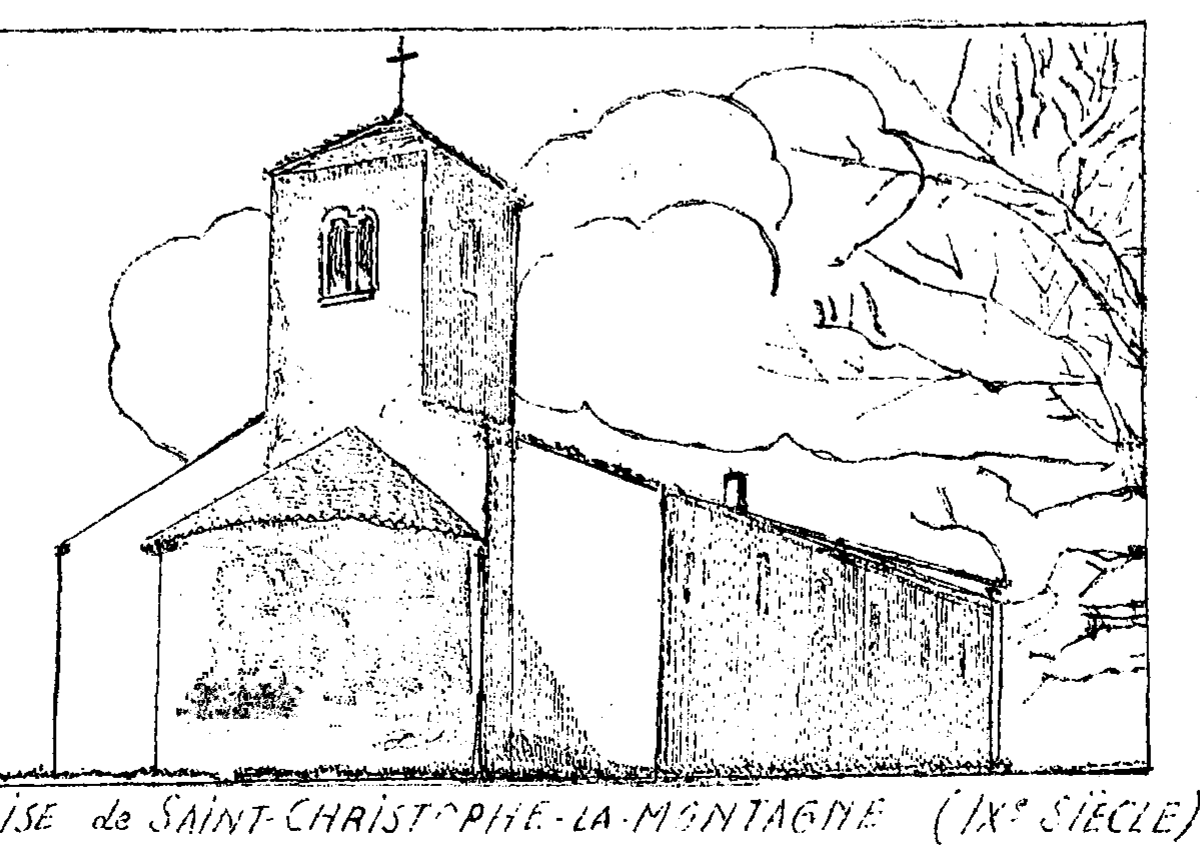
\includegraphics[width=0.55\textwidth]{Illustrations/illus-cures-saint-christophe.png}
\end{figure}

% --- Page imprimée 124 — vue 127
\begin{figure}[ht]\centering
    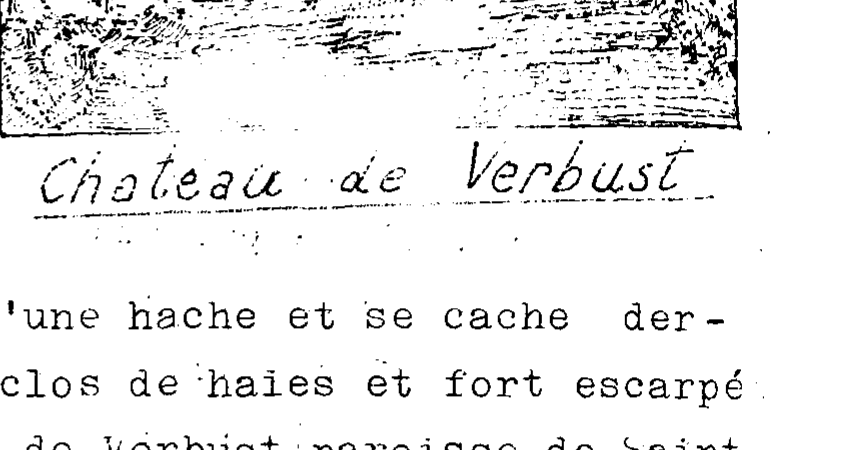
\includegraphics[width=0.48\textwidth]{Illustrations/illus-cures-verbust.png}
\end{figure}

Les mœurs révolutionnaires n'avaient que trop pénétré dans nos populations de campagne et les caractères violents trouvaient dans le souvenir des scènes dont ils avaient pu être témoins, des modèles pour satisfaire leurs vengeances.

Cet homme connaissait parfaitement les habitudes du saint curé : les jours de son voyage à St-Christophe, l'heure de son retour.

Aveuglé par la passion, il s'arme d'une hache et se cache derrière un arbre sur le bord du chemin clos de haies et fort escarpé qui va du hameau de la Forest à celui de Verbust, paroisse de Saint Mamert.

Tout allait à souhait ; il faisait noir, le silence était absolu, aucun témoin du crime n'était à craindre à cette heure. Mr Trouilloux arrive et le misérable s'apprête à se précipiter sur lui pour lui trancher la tête. Mais, ô prodige ! Mr Trouilloux n'est pas seul. Un grand nombre de personnes forment comme une longue file de chaque côté de lui. Il semble présider une procession. La hache tombe des mains du coupable ; il s'enfuit épouvanté jusque dans sa maison. Le remords s'empare de lui ; il raconte aux personnes de la maison et son dessein et ce qu'il a vu. Celles-ci viennent à Ouroux quelques jours après, s'informent quels étaient ceux qui accompagnaient Mr le Curé à son retour de St-Christophe, tel jour, à tel endroit, à telle heure. Mr Trouilloux n'avait rien vu et était absolument seul n'ayant à la main que son chapelet qu'il récitait pour les âmes du purgatoire, avoua-t-il ensuite.

Tous ceux qui eurent connaissance de ce fait extraordinaire, crurent que cette foule qui entourait Mr Trouilloux et le préserva d'une mort certaine n'était autre que les âmes du Purgatoire à l'intention desquelles il disait son chapelet.

Mr Trouilloux sentant ses forces décliner, voulut mettre ordre
% --- Page imprimée 125 — vue 128 (suite)
à ses affaires temporelles. Par son testament du 5 Novembre 1817, reçu par Plasse notaire à Ouroux, il laisse à la paroisse qu'il avait si longtemps administrée des témoignages précieux de son affection et de son dévouement. Indépendamment des messes qu'il ordonne être dites pour le repos de son âme, il prie les autorités de la commune de le faire inhumer sous le seuil de la grande porte de l'église. Son vœu fut réalisé. Le 6 Septembre 1866, les réparations faites au pavé de l'église nécessitèrent l'ouverture de son tombeau. Le corps était dans un état de décomposition complète. Mr Bouteille voulut conserver le crucifix qu'on avait placé entre ses mains au moment de sa mort. Ses ossements furent replacés sous la nouvelle dalle qui sert de seuil à l'entrée de l'église ; le crucifix est conservé religieusement à la cure.

Non content d'avoir fait des dons généreux à la Fabrique et au Bureau de Bienfaisance, il légua au grand séminaire de Lyon une rente de cent cinquante francs qui lui était due par Mr Lardet curé de Trivy (S \& L) à la charge de l'employer au profit de ses parents ou des pauvres de la commune d'Ouroux qui voudraient entrer dans les ordres sacrés. Nous n'avons au sujet de ce legs aucun renseignement. Peut-être n'a-t-il jamais été exécuté.

Nous verrons enfin, lorsque nous traiterons la question des écoles dans la paroisse quelle fut la générosité de Mr Trouilloux à leur égard. Disons seulement que si Mr Guillin fut le premier qui s'efforça d'introduire à Ouroux l'enseignement élémentaire, Mr Trouilloux en fut, lui, le vrai organisateur. C'est grâce à ses libéralités que notre paroisse voit ses enfants confiés aux soins dévoués d'une Congrégation qui a fait un bien aussi sensible au milieu de nous.

Mr François Trouilloux mourut le 20 Janvier 1818 âgé de 74 ans, après avoir été neuf ans vicaire et quarante ans curé de la paroisse. Il fut inhumé, avons-nous dit, selon sa volonté expresse, sous la grande pierre de l'entrée de l'église "pour garder, ajoute Mr Polloce, dans l'acte mortuaire, les portes du sanctuaire comme il l'avait fait pendant sa vie et reprocher hautement leur impiété à ceux qui osent profaner ce lieu respectable".

Furent présents à ses obsèques : MM. Bouillard, curé de Trades, Canard
% --- Page imprimée 126 — vue 129 (suite)
curé de St-Christophe la Montagne, Pras curé de Monsols, Vermorel curé de St-Jacques-des-Arrêts, Collonge curé d'Avenas, Chuzeville curé des Ardillats, Polloce vicaire d'Ouroux.

XXVIII-Pierre Marie Polloce qui devait succéder à Mr Trouilloux faisait suivre sa signature dans l'acte de décès de ces mots qui sont le plus bel éloge de la vertu du vénérable vieillard : "je fus témoin de ses vertus pendant deux ans et cinq mois ; puissé-je les retracer dans ma conduite". Son vœu, nous pouvons le dire à cette heure se réalise complètement. Mr Polloce ajouta un nom de plus à la liste déjà longue des prêtres zélés qui desservirent notre paroisse.

Pierre Marie Polloce, fils de Claude Polloce et de Benoîte Veaux naquit au hameau du Crozet commune de Poulle, le 22 Avril 1787 et fut baptisé le même jour. Son enfance s'écoula au milieu des tristesses et des persécutions de la Grande Révolution et nous savons que sa famille se distingua entre toutes par son zèle à maintenir la foi intacte autour d'elle et souvent sa maison servit de refuge et d'asile aux prêtres fidèles à leur devoir. Dieu récompensa le dévouement de ce père chrétien en appelant à l'état ecclésiastique un de ses enfants.

Mr Polloce fut nommé vicaire à Ouroux au commencement du mois d'Août de l'année 1815. À la mort de Mr Trouilloux il fut appelé par l'autorité épiscopale à prendre sa succession. Pendant 38 ans, il devait consacrer à la paroisse d'Ouroux son énergie et son zèle.

Bien des choses étaient en souffrance par suite de l'âge avancé et des infirmités qui avaient mis Mr Trouilloux dans l'impossibilité de subvenir à tous les besoins et surtout de réparer les suites désastreuses de la persécution. Mr Polloce se mit immédiatement à l'œuvre.

Il s'occupa, comme ses prédécesseurs, de donner au culte toute la splendeur possible, sans négliger pour cela le bien des âmes pour lesquelles il eut une affection toute spéciale. En 1818 il fit construire le maître-autel actuel et le retira du fond de l'abside où il avait été placé anciennement pour le mettre sous la coupole où il se trouve aujourd'hui.

% --- Page imprimée 127 — vue 130
Vers 1830 et les années suivantes, il fit disparaître les chapelles qui occupaient les deux nefs latérales, pour donner aux fidèles un plus grand espace et commença en même temps plusieurs réparations à la cure, qui était dans un état de délabrement impossible à décrire. En 1833, le 17 Octobre, il érigeait dans l'église de nouveaux tableaux du chemin de croix. Enfin en 1839 il fit faire à Mr Burdin, fondeur à Lyon, deux cloches pesant l'une 750 kilos et l'autre 500 kilos.

En 1844 se trouvant dans l'impossibilité de desservir seul sa paroisse il demanda un aide. Ce fut Mr Morétain qui fut appelé à lui prêter son concours comme vicaire. Le vicariat ne devait être autorisé qu'en 1848.

Il serait trop long d'entrer dans tous les détails de l'administration de Mr Polloce, d'énumérer toutes les réparations, tous les achats qu'il fit. Qu'il nous suffise d'ajouter qu'en 1855 il acheta un orgue de 6 jeux au prix de 1900 francs et le plaça à l'église derrière l'autel. Mr Dutruge, ayant quitté la paroisse pour aller à Fleury, Mr Bouteille ne put lui donner un successeur comme organiste. Il revendit l'instrument. Cet orgue réparé fut installé à Cluny.

Enfin ce fut encore Mr Polloce qui fit transporter le cimetière, au nord du bourg, sur la route du Razay. Jusqu'à là les morts avaient été inhumés ou dans l'église ou autour de l'église elle-même. Mais à la suite des changements survenus dans la disposition de la place, toutes les eaux s'écoulaient dans le cimetière et rendaient le creusement des fosses impossible. Le nouveau cimetière fut bénit le 2 Novembre 1854. Mr l'Abbé Mahuet Joseph né à Ouroux fut le prédicateur choisi pour la circonstance.

Mr Polloce fut appelé à diriger notre paroisse pendant la période la plus troublée peut-être, qu'elle ait eu à traverser. Pendant la Révolution elle fut admirable de religion et d'énergie ; mais il n'en est pas moins vrai que la jeunesse avait reçu une éducation très incomplète. Certaines familles avaient conservé et entretenaient entre elles des inimitiés qui se faisaient jour à tout instant, sous une forme ou sous une autre. L'esprit d'indépendance était fomenté par quelques meneurs qui tenaient à diriger jusqu'à un certain point la paroisse, imposer leurs volontés et profiter des désordres pour leur
% --- Page imprimée 128 — vue 131 (suite)
bien personnel. Les autorités de la commune elles-mêmes semblaient les exciter par leurs exemples, souvent même par leur appui formel.
En 1848 un vent de révolte souffla dans la vallée. À peine la République était-elle proclamée que quelques énergumènes montèrent au clocher, sonnèrent le tocsin et organisèrent la Garde Nationale. 34 fusils qui se trouvaient à la mairie furent confiés à des armuriers pour être réparés. Les plus exaltés envahirent la cure et demandèrent à boire. Quatre d'entre eux allèrent même jusqu'à Germolles et forcèrent Mr le Curé de leur ouvrir sa cave. Un voisin d'une taille herculéenne vint mettre fin, heureusement, à ses velléités de gaspillage et la petite troupe rentra dans ses cantonnements.
C'était bien là un indice du travail qui s'était fait dans les esprits ; il faut l'avouer cependant, ceux qui voulaient ainsi jouer aux révolutionnaires n'habitaient que depuis quelques années dans la paroisse ou bien avaient perdu toute considération autour d'eux. Tous ont péri misérablement. Comme le leur avait dit Mr Polloce, ils sont morts sur la paille.
Mr le curé tint tête à l'orage et la seconde république ne fit, comme ailleurs du reste du bruit qu'au commencement.
Néanmoins les rapports entre le conseil municipal et le conseil de fabrique ne se détendirent jamais complètement. Le dissentiment éclata en 1855 pour un motif qui peut paraître en lui-même insignifiant, mais que Mr Polloce devait regarder comme important.
En 1827 le maire de la commune ne trouvant pas de local convenable pour en faire une salle de mairie demanda à Mr le curé, de concert avec MM. les Fabriciens, l'autorisation d'affecter à cet effet une chambre de la cure moyennant une redevance annuelle de vingt F, redevance qui, d'ailleurs ne fut payée que les deux premières années. Une porte extérieure s'ouvrant sur la place permettait de communiquer avec le dehors. C'était là pour la cure une réelle servitude. Souvent aussi le bruit qui se faisait dans cette chambre, située en face de la grande porte de l'église était pour les fidèles un sujet inévitable de distractions. Mr Polloce invita le Conseil Municipal par l'intermédiaire du maire à rétablir cette chambre dans son état primitif et à se procurer un local dans une situation moins oné
% --- Page imprimée 129 — vue 132 (suite)
reuse et moins incommode pour la cure.

Le conseil refusa alléguant la possession immémoriale. Le conseil de fabrique en appela à l'autorité supérieure et à la suite d'un exposé fidèle et détaillé de la situation, le sous-préfet de Villefranche ordonna au maire d'Ouroux d'avoir à reconnaître les droits au curé et à remettre l'appartement à la disposition de ce dernier.

L'amour propre d'un certain nombre de membres avait été froissé ; ils ne devaient jamais pardonner à Mr Polloce le triomphe qu'il avait obtenu. Aussi les mécontents trouvèrent-ils bientôt l'occasion de poursuivre leurs vexations.

La place actuelle servait autrefois de jardin à la famille Duligier. Un chemin ou plutôt une sorte de sentier donnait accès à l'église. Le dernier membre de cette famille, Jean Antoine Marie Duligier le céda à la commune qui le convertit en place publique. La place était néanmoins fort incommode par suite de la pente très prononcée du sol. L'église n'était donc enterrée dans aucune de ses parties.

En 1848 malgré les protestations énergiques de Mr Polloce quelques particuliers profitant des désordres du moment prirent la liberté d'élever le chemin allant de la rivière à la grande rue passant près du chœur de l'église. Les réclamations furent regardées comme non avenues.

Plus tard lorsqu'on eut construit le chemin de grande communication d'Ouroux à Fleurie, il fallut de toute nécessité ou exhausser les abords de la place ou bien faire contourner le bourg par une nouvelle route. Le conseil de fabrique s'opposa énergiquement à l'exécution du projet de la municipalité qui consistait précisément à élever le chemin longeant l'église. Mr Poloce lui-même fit démarches sur démarches pour sauvegarder les intérêts matériels et religieux de la paroisse. Mais il ne put avoir gain de cause, et il vit avec douleur l'église rendue insalubre, inabordable à la suite de cette quantité énorme de matériaux que l'on vint déposer contre ses murs, à quelques mètres à peine. Aujourd'hui elle a perdu son cachet monumental ; elle est d'un accès difficile et l'humidité considérable que ces matériaux engendrent cause des dégâts irréparables pour les
% --- Page imprimée 130 — vue 133 (suite)
peintures et les murs eux-mêmes.

Mr Polloce, par suite de ces oppositions systématiques, crut que désormais tout ministère dans la paroisse cesserait d'être fructueux. Il demande donc à l'autorité diocésaine de se retirer. Son Éminence le Cardinal de Bonald au courant des luttes du vénéré curé voulut le récompenser et le nomma chapelain à Notre-Dame de Fourvière.

Mr Polloce quitta la paroisse d'Ouroux le 15 Octobre 1857 après l'avoir administrée deux ans comme vicaire et trente huit ans comme curé. Il mourut en 1862 et fut inhumé au cimetière de Loyasse dans la concession achetée pour les prêtres.

Mr Polloce conserva toujours un souvenir affectueux pour Ouroux ; il semble même qu'il s'était attaché à cette paroisse à proportion des difficultés qu'il y avait rencontrées. Souvent ses anciens paroissiens allaient à Fourvière le revoir et dans un entretien affectueux il se plaisait à leur rappeler les anciens souvenirs, s'informant des moindres détails qui toujours l'intéressaient ; souvent il se laissa aller jusqu'à avouer aux plus intimes qu'il regrettait d'avoir quitté Ouroux. La paroisse tout entière du reste le regardait comme un saint et lui conserva jusqu'à sa mort un attachement sincère. Les tracasseries qu'il eut à subir n'avaient pour auteurs des hommes de peu de considération qui voulaient entraver l'action du prêtre mais qui respectaient et vénéraient l'homme.

Je ne saurais oublier, en terminant cet article, l'impulsion qu'il donna dans sa paroisse aux vocations religieuses. Mr Trouilloux comme tous les prêtres zélés, comprit au sortir de la Révolution qu'il fallait des prêtres pour remplacer les vides nombreux faits par la mort ou les persécutions. Sept prêtres lui furent redevables de leur vocation à l'état ecclésiastique ; quatre autres furent ordonnés sous Mr Polloce.

XXIX-Jean Claude Benoit Bouteille était "né à Larajasse le 5 novembre et appartenait à une famille nombreuse qui jouit d'une considération méritée. Ses premières études furent dirigées par un saint prêtre Mr Roux devenu plus tard professeur de dogme ; il passa ensuite élève à Verrière, puis à l'Argentière dont il sortit pour en
% --- Page imprimée 131 — vue 134 (suite)
trer au grand séminaire de Lyon.

Ordonné prêtre en 1840, il fut aussitôt nommé vicaire à Perreux. Il y resta 17 ans. Mr Bennetton d'abord et après lui Mr Gorand, curés de cette paroisse guidèrent ses premiers pas dans le ministère. Il sut si bien profiter des leçons de ces prêtres vénérables qu'il s'attira en peu de temps l'estime et l'affection de tous les habitants de Perreux. Les souvenirs qu'il a laissés sont encore vivants. Dès le début de sa carrière ecclésiastique il se montra tel qu'il fut toujours : pieux, travailleur, infatigable, austère pour lui-même autant que doux et bienveillant pour les autres, joignant à une entière fermeté dans les principes, les ressources d'une charité toujours disposée à excuser.

En 1857 ses supérieurs hiérarchiques le jugèrent mûr pour la direction d'une paroisse. Il l'était en effet. Le poste de Saint-Antoine d'Ouroux était vacant par suite de la retraite à Fourvière du vénéré Mr Polloce. Mr Bouteille fut appelé à le remplir. Il accepta.

Son administration fut celle d'un homme intelligent et entendu. Sous sa direction, la vieille église qui s'en allait en ruines fut appropriée, ornée et meublée avec un goût qui lui fait honneur.

Qui dira le bien moral dont il fut l'auteur. Il connaissait ses paroissiens, comme un père connaît ses enfants. Il donnait à tous les conseils de son expérience. Tous les recevaient avec plaisir parce qu'ils étaient ceux d'un homme de jugement et de cœur.

Ses instructions pastorales étaient de petits chefs-d'œuvre de touchante simplicité. Les étrangers qui avaient le bonheur d'y assister en sortaient frappés et ne manquaient pas d'en faire la remarque

On retrouvait partout en lui, dans sa personne comme dans son âme un mélange de bonté et de gravité. Faut-il s'en étonner ? Tous ses actes lui étaient dictés par un cœur naturellement bon que l'exercice du ministère avait rendu plus tendre encore. Il savait que le prêtre est le ministre du Dieu venu sur la terre pour compatir à nos faiblesses et à nos misères. Il savait que le cœur du prêtre doit être un asile toujours ouvert à ceux qui souffrent et cette science, l'une des assises de notre religion, sa charité l'avait mise en pratique. Ce fut la seule arme qu'il opposa à cet esprit de socialisme et d'irré
% --- Page imprimée 132 — vue 135 (suite)
ligion qui avait souffert dans sa commune comme partout ailleurs. Il le subit comme on subit un ouragan, sachant bien que le dernier mot est à Dieu qui ramène le calme quand bon lui semble.

C'est au service de sa charité et en allant voir les malades qu'il contracta la maladie dont il devait souffrir pendant plusieurs années et qui termina trop tôt une vie aussi précieuse. Il mourut dans sa 65ème année, entouré des siens, entouré de toute sa paroisse laissant à tous le souvenir de ses vertus.

Cette courte notice qui a pour auteur Mr Berloty Adrien, fut lue par lui sur la tombe de Mr Bouteille et parut dans l'Echo de Fourvière le 9 Aout 1879. Elle offre un résumé succinct, mais très fidèle d'une existence consacrée au salut des Âmes. Mon sujet exige néanmoins que j'entre dans quelques détails qui nous feront mieux comprendre toute la justesse et l'énergique précision de ces quelques lignes.

Le jour même où Mr Polloce était nommé chapelain à Fourvière, le 15 Octobre 1857, Mr Bouteille était installé à Ouroux. Placé à la tête de notre paroisse, il devait s'y distinguer par une prudence remarquable et une sagesse consommée. Suivant en cela les exemples de ses prédécesseurs, ses premiers soins furent encore pour l'église ; et il faut le reconnaître, il trouva dans la générosité inépuisable du nouveau propriétaire de Gros-Bois, Mr Berloty, une ressource que la Fabrique ne pouvait lui offrir. Nous verrons au chapitre concernant l'église en quoi consistèrent les réparations que Mr Bouteille fit exécuter ; qu'il nous suffise de dire que nous lui devons la chaire et les confessionnaux, les magnifiques chandeliers romans du maître-autel, les quatre lustres d'un si gracieux effet. Ce fut lui qui fit peindre le chœur avec ce goût délicat qui le distinguait en toutes choses.

Mr Bouteille préoccupé à juste titre de l'instruction des enfants qui lui étaient confiés, témoin des difficultés sans nombre qui résultaient pour eux des changements fréquents qui avaient lieu pour les instituteurs, secondé d'ailleurs par un maire religieux et universellement estimé, résolut de confier à des frères la direction de l'école de garçons. Il s'adressa à cet effet à l'institut

% --- Page imprimée 133 — vue 136
Petits Frères de Marie qui mit à sa disposition un religieux zélé, frère Edwin avec deux aides. La divine Providence qui ne jugea pas la paroisse digne d'une direction aussi éclairée devait les rappeler bientôt ; du moins épargna-t-elle à Mr Bouteille la douleur de les voir partir après cinq ou six ans d'efforts et de luttes.

Mr Bouteille fut surtout un homme de conseil et c'est à ce titre qu'il acquit autour de lui une réputation qui s'étendit bientôt au loin et fit qu'on vint le consulter de toute part. Tenu au courant de toutes les lois, il savait à propos ménager les ententes, arrêter les procès, parfois aussi donner des conseils sur la direction d'une ferme, l'entreprise d'une construction. Et des hommes haut placés, dont nous avons eu la correspondance entre les mains, ne dédaignèrent pas de s'adresser souvent à lui à ce sujet. Précieux intermédiaire qui par son influence et sa sagesse pouvait être d'un réel secours pour traiter avec impartialité les intérêts des maîtres et de leurs nombreux fermiers.

Ajoutez à cela une énergie, un sang-froid qui ne l'abandonnèrent jamais, même au milieu des dangers les plus graves, comme il le fit bien voir dans les incendies qui dévastèrent à deux reprises le bourg d'Ouroux et le village du Razay. Là en particulier il se distingua à un tel point qu'il reçut du Ministère de l'Intérieur un éloge public, bien mérité. Le diplôme constatant son dévouement dans cette circonstance fut trouvé dans ses papiers après sa mort et remis à sa famille ; sa modestie lui avait fait tenir caché ce témoignage officiel de son courage.

Au point de vue spirituel, il donna à la paroisse une direction excellente. Bien des abus tombèrent comme par enchantement, tant ses exhortations étaient persuasives et entraînantes. Sans froisser jamais personne, il savait lorsque les circonstances l'exigeaient, élever la voix, soutenir le parti du bien, et ce fut grâce à cette prudence qu'on ne put jamais prendre en défaut, qu'il opposa une digue au torrent révolutionnaire qui menaça notre vallée.

Plusieurs fois l'Administration diocésaine, connaissant le mérite de Mr Bouteille le chargea de missions importantes et délicates. Il fut spécialement désigné pour faire les enquêtes nécessitées par
% --- Page imprimée 134 — vue 137 (suite)
l'établissement projeté des deux paroisses de Saint-Mamert et du Vieux-Château sur la commune de Cenves.

Disons enfin qu'il fut nommé délégué cantonal et à ce titre chargé de l'inspection des écoles.

Doué d'une santé robuste, ni distances, ni fatigues, rien ne l'arrêtait. Il contracta un asthme d'une violence qui eut bientôt raison de sa forte constitution. Vers la fin de Juillet 1879 une crise plus violente le força de s'aliter pour ne plus se relever. Le Dimanche 3 Août, à 4 heures du soir, il rendait son âme à Dieu, en présence d'un grand nombre de ses paroissiens. Ses obsèques eurent lieu le mardi suivant. Tous se firent un devoir de lui témoigner sa reconnaissance. Trente deux prêtres voulurent attester par leur présence les hautes qualités de celui qui venait de les quitter.

Il fut inhumé dans le cimetière de la paroisse, au pied de la grande croix. Le monument qui lui a été élevé est le fruit d'une souscription.

------------------------------------------------------------------------
N.B. Mr l'Abbé Odouard, auteur de l'Histoire d'Ouroux termine le chapitre "Curés d'Ouroux" avec le nom de l'Abbé Bouteille. Pour compléter ce chapitre, nous dirons quelques mots des curés qui administrèrent la paroisse d'Ouroux jusqu'à nos jours.
------------------------------------------------------------------------

XXX-Étienne Savoie fut curé d'Ouroux de 1879 à 1888. Il était originaire de Vauxrenard. Il était remarquable dans sa prédication au cours de laquelle, bien des fois, les femmes ne pouvaient retenir leurs larmes.

XXXI-Ferdinand Aubert desservit notre paroisse pendant onze ans, de 1888 à 1889. Prêtre très charitable il travailla à l'embellissement de son église, en faisant réparer les autels de la Ste Vierge et de St-Antoine, ainsi que les plâtres et les peintures. Mr Aubert organisa aussi un grand pèlerinage paroissial à Paray-le-Monial. On allait prendre le train à Clermain.

XXXII-Félix Rambaud arriva à Ouroux le 1er décembre 1899. Il y demeura quatre années. C'était un prêtre très estimé, d'allure bourgeoise, mais familier et dont on regretta le départ.

% --- Page imprimée 135 — vue 138
XXXIII - Jean Claude Planus resta pendant 5 années curé d'Ouroux de
1903 à 1908, avant d'aller fonder la paroisse de Montplaisir-la Plai-
ne. C'était un grand prédicateur, au timbre de voix puissant. Il é-
tait très bon avec ses paroissiens. Prêtre du Prado, il vivait très
pauvrement, se contentant que du strict nécessaire en mobilier et
en nourriture. C'est sous son ministère qu'eut lieu cette période
assez mouvementée de la Sécularisation et des Inventaires des biens
d'église.

On sait qu'avant la séparation de l'Église et de l'État, on vi-
vait sous le Concordat de Napoléon Ier. Le gouvernement choisissait
les évêques qui étaient investis par Rome de leurs pouvoirs spiri-
tuels et le clergé recevait un traitement qui était la compensation
des anciens biens supprimés par la Révolution. Une fois la loi de
Séparation votée (9 décembre 1905) le Concordat se trouvait suppri-
mé et supprimé aussi le traitement du clergé ou budget des cultes.

Mais qu'allaient devenir les biens appartenant aux évêchés et
aux paroisses (menses ou fabriques) ? La loi décidait qu'on devrait
fonder partout des "associations cultuelles" qui recevraient la
propriété de tous ces biens à condition de se former tout de suite.
Si elles ne l'étaient pas au bout d'un an, tous les biens seraient
confisqués par l'État. La question fut portée à Rome, au nouveau pa-
pe Pie X. Mais dans un geste qui parut alors pour quelques-uns un
geste d'intransigeance, mais qui, avec le recul du temps, apparaît
déjà comme un des plus beaux et des plus nobles de l'histoire, Pie X
préféra sacrifier tous les biens de l'Église de France et rejeta
cette loi qui brisait insidieusement la Constitution même de l'É-
glise. Accepter les associations cultuelles, telles qu'elles sont,
disait-il, "nous ne le pouvons pas sans trahir la sainteté de notre
charge, sans amener la perte de l'Église de France"

À partir de ce moment, ce fut une vraie curée : l'État s'empara des
biens des fabriques, des séminaires, des fondations pieuses léguées
par les défunts pour faire dire des messes, des caisses de retraite
pour les vieux prêtres. Cette spoliation odieuse fut l'œuvre mar-
quante d'Aristide Briand.

% --- Page imprimée 136 — vue 139
Conformément à l'article 3 de la loi de Séparation, le Gouvernement faisait procéder aux inventaires par l'Administration des Domaines. Cette opération, qui apparut aux catholiques comme un prélude de la confiscation, suscita une si vive émotion que les agents du fisc se heurtèrent parfois à des résistances si violentes qu'il leur fallut faire appel à la force armée. À Paris, dans les grandes villes et même dans beaucoup de villages, notamment en Bretagne et dans le Nord, il y eut de terribles bagarres.

À Ouroux tout se passa dans le calme. Tout d'abord à la nouvelle du projet de la loi de séparation, toute la France Chrétienne s'est levée pour protester contre cette atteinte aux droits des Français. Les habitants d'Ouroux n'ont pas été en retard pour faire entendre leurs voix ; les feuilles de pétition se sont couvertes de 465 signatures, 217 d'hommes et 248 de femmes.

Cependant l'opération sacrilège de l'inventaire de notre église s'est accomplie à Ouroux au milieu des plus vives protestations et a donné lieu à une belle manifestation religieuse. L'agent du gouvernement n'a pu terminer son travail à sa première visite le 9 mars 1906. Il s'est troublé à la vue des nombreuses personnes rassemblées à l'église qui avaient voulu être témoins de cette iniquité pour la raconter plus tard à leurs petits enfants et il s'est sauvé en toute hâte ! Mais comme l'opération était inachevée il est revenu 15 jours plus tard. Après de nouvelles protestations, tout a été fait en silence et en quelques minutes.

Nous lisons, dans le registre des délibérations de la fabrique d'Ouroux trois protestations, la première du curé contre l'inventaire de la Mense Curiale, la seconde du curé et des Fabriciens contre l'inventaire de l'église et la troisième de Pierre Montel, président du bureau des marguilliers de la fabrique de St-Antoine d'Ouroux contre l'inventaire.

Pour ne pas être trop long, relevons ici, seulement la seconde.

Monsieur,

Après la lettre que notre St Père le Pape vient d'adresser le 11 février 1906 à l'Église catholique de France, dans laquelle il condamne formellement comme injuste, la loi de Séparation et en attendant que ce même pontife nous dise ce qu'il pense de la dévolution des biens prescrits par ladite loi, moi curé et nous Membres du Con
% --- Page imprimée 137 — vue 140 (suite)
seil de fabrique, nous sommes obligés en conscience de vous opposer une résistance au moins rigoureusement passive et de vous laisser l'entière responsabilité de l'inventaire que vous avez l'intention de faire.

Nous resterons ici pendant votre opération, non pour donner une adhésion quelconque, mais parce que nous sommes chez nous et que nous avons le devoir de veiller aux biens de notre église dont la garde nous a été légitimement confiée.

Ici tous les meubles nous appartiennent : ornements, autels, vases sacrés, croix, chaire, confessionnaux, fonts baptismaux, chandeliers, bannières, bancs, calorifères et autres.

Tout, absolument tout a été mis gracieusement à la disposition du culte catholique par des paroissiens en particulier ou en collectivité, qui se réservent le droit d'en revendiquer la propriété à l'avenir s'il y a lieu.

Nous protestons avec la même énergie et en revendiquant tous nos droits contre l'inventaire de la mense curiale et des autres biens dont la gestion nous a été confiée. Ces biens que nous administrons sont la propriété de notre église, car ils nous ont été donnés uniquement pour son service par quelques bienfaiteurs catholiques.

En conséquence, moi curé de la paroisse de St-Antoine d'Ouroux et nous, membres du conseil de fabrique, administrateurs des biens de notre église nous ne céderons à personne aucun de ces biens, à moins d'un ordre formel de nos supérieurs ecclésiastiques qui sont le Souverain Pontife et Monseigneur l'Archevêque de Lyon.

En protestant de toutes nos forces contre votre opération, nous faisons notre devoir ; maintenant puisque violence nous est faite par la loi, accomplissez votre œuvre comme bon vous semblera.

Nous demandons que cette protestation soit insérée au procès-verbal. Ouroux le 9 mars 1906

Signés : Planus, curé ; Voland ; Chagny ; Gonnet ; Chevalier.

Quelques mois plus tard, un arrêté du préfet daté du 13 décembre 1906, envoyé par le brigadier de la gendarmerie de Monsols, à Mr Planus, curé desservant la paroisse d'Ouroux et à Mr Pierre Montel président du Bureau des marguilliers, notifiait déjà qu'à partir de ce jour tous les biens appartenant à la mense curiale d'Ouroux et à la fabrique de l'église d'Ouroux étaient placés sous séquestre.

L'abbé Planus reçut, daté du 19 décembre 1906, une circulaire envoyée par le Receveur des Domaines à la résidence de Monsols, lui ordonnant de "vouloir bien lui remettre ou lui faire parvenir dans le délai de huit jours et sous peines de droit, les espèces, valeurs, titres et autres documents quelconques dont il serait dépositaire"

À la suite de ces deux notifications le Curé Planus répondit la lettre suivante

% --- Page imprimée 138 — vue 141
Monsieur le Receveur
J'ai hésité à répondre à votre notification recommandée.
Je le fais cependant pour vous dire que ma conscience de catholique et de prêtre m'interdit formellement de vous faire parvenir les titres et autres demandés.
L'armoire fabricienne est à trois clés. J'en possède une et je vous déclare carrément que je ne m'en servirai jamais, pour coopérer à la spoliation des biens de notre église, dépôt sacré qui m'a été confié. Du reste ce que vous demandez m'est défendu par le texte même du décret constitutif des fabriques, relatif à l'armoire à trois clés et par l'article 1247 du code. Je me refuse donc énergiquement à commettre un acte de lâcheté, absolument contraire à mes convictions, à ma dignité et à mes devoirs.
Tout est prêt dans ladite armoire. Si je suis présent à votre arrivée on vous opposera une résistance rigoureusement passive. Les clés se trouveront à portée du meuble et là seulement, après protestation, il vous sera possible de vous emparer de nos biens. Mais que nous fassions la moindre démarche pour vous les livrer nous-mêmes, jamais ! Ainsi nous pourrons être dépouillés par la violence, mais nous ne deviendrons pas prévaricateurs.
Veuillez agréer, monsieur le Receveur, l'expression de mon profond respect.
Signé : J. Cl. Planus, curé d'Ouroux
Ce n'est que le mercredi 21 Août 1907, dans l'après-midi, qu'eurent lieu à Ouroux, les opérations de prise de possession des titres et documents par le receveur de Monsols. La protestation suivante lui fut remise :
"Les membres de la fabrique de St-Antoine d'Ouroux, réunis à la veille d'une dissolution forcée, ordonnée par la loi de Séparation, condamnée par le Souverain Pontife, ont été d'avis d'adresser au Séquestre la protestation suivante :
"Nous membres du Conseil de Fabrique de St Antoine d'Ouroux, protestons avec toute l'énergie de nos volontés, et en catholiques convaincus, contre le dessaisissement de la gestion des biens de l'église et de la fabrique de St Antoine d'Ouroux, qui nous est imposé, contrairement à la volonté de la Sainte Église, catholique et romaine.
Nous déclinons toute responsabilité, relativement à la gestion de ces biens dans l'avenir.
Nous demandons qu'il nous soit remis une décharge des biens, titres et documents qui vont nous être enlevés.
Nous terminons en faisant profession de fidélité et de dévouement à l'autorité de Notre Saint-Père le Pape et de Son Éminence Monseigneur Coullié, notre bien-aimé Cardinal.
À Ouroux le 12 décembre 1906
Les membres du conseil de fabrique
Signés : Gonnet ; Montel ; Voland ; Chagny et Planus, curé.
Mr le Receveur des Domaines prit possession du contenu de l'armoire fabricienne. Avant de s'en aller il laissa une décharge
% --- Page imprimée 139 — vue 142 (suite)
écrite et signée de sa main de tout ce qu'il emportait et sur laquelle était d'abord mentionnée la protestation ci-dessus.
    Sans rentrer dans les détails, signalons cependant sommairement quels étaient les biens et les charges qui étaient à l'église et à la mense curiale d'Ouroux. Mr l'abbé Grapeloup en a laissé une attestation signée des membres du conseil de fabrique et de lui-même
    Comme Biens il y avait :
1/ deux titres de rentes sur l'État (25+13=38 fr de rente annuelle)
2/ un titre nouvel par Mr Cl. Gauthier, au profit de la fabrique (rente annuelle de 30 fr, payée par Alexandre Gauthier, propriétaire cultivateur, lieu de la Fuserie et répartie ainsi : 20 fr pour 10 messes par an et à perpétuité, 10 fr pour la fabrique)
3/ un titre nouvel par Messieurs Jacques Lapierre, meunier propriétaire, Benoit Dufour, propriétaire cultivateur, Benoit Tribolet, propriétaire cultivateur demeurant à St-Christophe la Montagne et débiteurs solidaires envers la fabrique d'Ouroux d'une rente perpétuelle de 83 fr 80 en espèces et de la redevance de 4/5 d'un poulet par an. Répartition de cette rente était 10 fr pour 5 messes par an et à perpétuité ; le reste à la fabrique. (Ce titre est dû au testament de Mr Trouilloux daté du 5 novembre 1817)
4/ une copie de donation consentie le 24 janvier 1771, par sieur Cl. Monnet, bourgeois demeurant à Jullié, au profit des pauvres de Jullié et d'Ouroux, moyennant fondation d'une messe annuelle et perpétuelle à la charge du bureau de bienfaisance d'Ouroux.
5/ le pré au-delà du pont de la Grosne, dit pré de la tannerie, acheté 1653 fr moitié par le Bureau de bienfaisance pour le service des religieuses St Joseph, moitié par la fabrique pour le service du curé (acte daté du 19 septembre 1826)
6/ le demi-arpent qui forme le pré touchant la cure et une partie du jardin en ligne droite partant du petit colombier au mur Joly qui a été acheté par Julien Chagny (qui l'avait acheté au gouvernement 10.000 livres après l'extinction de 7 feux) par Mr Jean Lardet et Benoit Laplasse d'Ouroux pour l'église de ladite paroisse
7/ le pré dit chenevis qui est au-dessous du vieux cimetière en allant vers la rivière
8/ un bois dit "de la fabrique" ou mieux "du curé" selon l'acte. Acheté par Mr de Guillin curé d'Ouroux du Seigneur Michel comte de Fautrière pour en laisser la propriété à ses successeurs (acte du 20 décembre 1746)
9/ l'église, la cure et le jardin dont il n'a été trouvé aucun acte.
    Comme Charges au total 16 Messes par an, comme il a été signalé ci-dessus.
XXXIV-Pierre Michard succéda à l'Abbé Planus comme curé d'Ouroux, pendant 10 ans, de 1908 à 1918. Comme son prédécesseur il connut durant son ministère quelques années douloureuses. Toutes les luttes intestines et religieuses, en France, se turent et tous les esprits, réalisant l'union sacrée, restèrent tournés vers le dénouement de
% --- Page imprimée 140 — vue 143 (suite)
l'effroyable drame qu'était la grande guerre de 1914-1918. Le curé Michard n'était pas un orateur comme le furent certains de ses prédécesseurs, mais il savait consoler et dire aux familles éprouvées le mot qui donnait de l'espoir ou bien qui faisait supporter chrétiennement une grande épreuve. Ses paroissiens le considéraient comme un saint prêtre.

XXXV-Joannes Gros fut curé d'Ouroux de 1918 à 1935. Il était natif de Villechenève. Sa prédication était remarquable, très concrète et courte. Certains paroissiens allaient uniquement à la messe pour l'écouter. C'est lui qui organisa dans la paroisse la Ligue catholique des femmes françaises. La paroisse d'Avenas n'avait pas de curé résidant depuis 1927, après le départ de l'Abbé Séon. Un ancien curé d'Avenas, alors curé de Vauxrenard, l'Abbé Élisée Morel (aujourd'hui moine à la Trappe des Dombes) desservit Avenas jusqu'en 1931. Pendant quelques années le curé Gros monta à Avenas, mais son état de santé rendant cette charge trop pénible, Avenas fut confié à l'Abbé Aulagnon, curé de St Joseph en Beaujolais. L'Abbé Gros, pour raison de santé se retira à Tarare où on lui donna une petite aumônerie.

XXXVI-Claude Delvaux curé d'Ouroux de 1935 à 1944. Mr Gros, malade sur ses dernières années passées à Ouroux était porté à négliger un peu l'entretien de son église et de sa cure. Son successeur aménagea la cure, fit quelques restaurations à l'église, installa une madone au-dessus des Friats. De nouveau il y eut une belle chorale. Des anciennes coutumes furent rétablies telles les belles cérémonies de la Fête Dieu, la lecture de la Passion pour les fruits de la terre, etc. Mr l'abbé Delvaux fut nommé ensuite curé-archiprêtre de la paroisse St-Nicolas, à Beaujeu.

XXXVII-Jean Magat originaire de Fournaux (Loire) fut installé par Mgr Merlier le 16 Juillet 1944. C'est lui qui lança les mouvements d'Action Catholique dans la paroisse (J.A.C. ; JACF et M.F.R.) Il fit reparaître le Bulletin paroissial qui avait cessé de paraître avec la grande guerre, du temps du curé Michard. Il travailla aussi à l'embellissement de l'église, organisa des Kermesses, etc.

XXXVIII-Joseph Aubonnet, né à Poule arrivé le 13 juillet 1948.
